%some-literature review


In the last few decades, several scientists have modeled the dynamics and ecological impact of marine aggregates \cite{jackson_aggregation_1998, kiorboe_mechanisms_2002}. 
Their effects on bacterial transport \cite{jackson_simulation_1989} and algal bloom \cite{jackson_model_1990} have been described in models that use simplified descriptions of the aggregates' settling speeds. Moreover, accumulation of aggregates in thin layers where the ambient fluid is stratified have been reported \cite{macintyre_accumulation_1995, alldredge_occurrence_2002} and more recently modeled experimentally \cite{prairie_delayed_2013}, analytically \cite{camassa_retention_2013}, and computationally \cite{panah_simulations_2017}. Understanding the formation and persistence of these thin layers is ecologically important. 
Therefore, in this chapter, we discuss the dynamics of settling marine aggregates in a density stratified fluid. 
%---------------------------------------------------------
\par
Instead of constant density $\rho$, we suppose the background fluid density varies linearly in the vertical direction,
\begin{equation}
\rho_{bg}(z) =  \rho_0 \left(1 - \gamma z \right),
\label{eq_rho_bg}
\end{equation}
where $\rho_0$ is the fluid density where the aggregate's center of mass is located at rest, and $\gamma > 0$ is constant.
Over the time $t$, some perturbations, $C(\vec{y},t)$, occur due to the concentration, $\tilde{S}(\vec{y},t)$, difference between the background fluid and settling aggregate,
\begin{equation}
C(\vec{y}, t) =  \tilde{S}(\vec{y},t) - \rho_{bg}(z).
\label{eq_perturb_C}
\end{equation}
From equations (\ref{eq_rho_bg}) and (\ref{eq_perturb_C}), we can establish the fluid density variation over time,
\begin{equation}
	\rho(\vec{y},t ) 
	= \rho_{bg}(z) +  \alpha \rho_0 C(\vec{y},t) 
	 = \rho_0 \left( 1 - \gamma z  + \alpha  C(\vec{y},t) \right),
\label{eq_density}
\end{equation}
where the non-zero constant $\alpha $ describes type of solute. Knowing that the concentration is the amount of mole per volume, the density of the fluid would differ by the type of solute or chemicals with the same amount of molecules.
\begin{figure}[ht]
	\begin{center}
	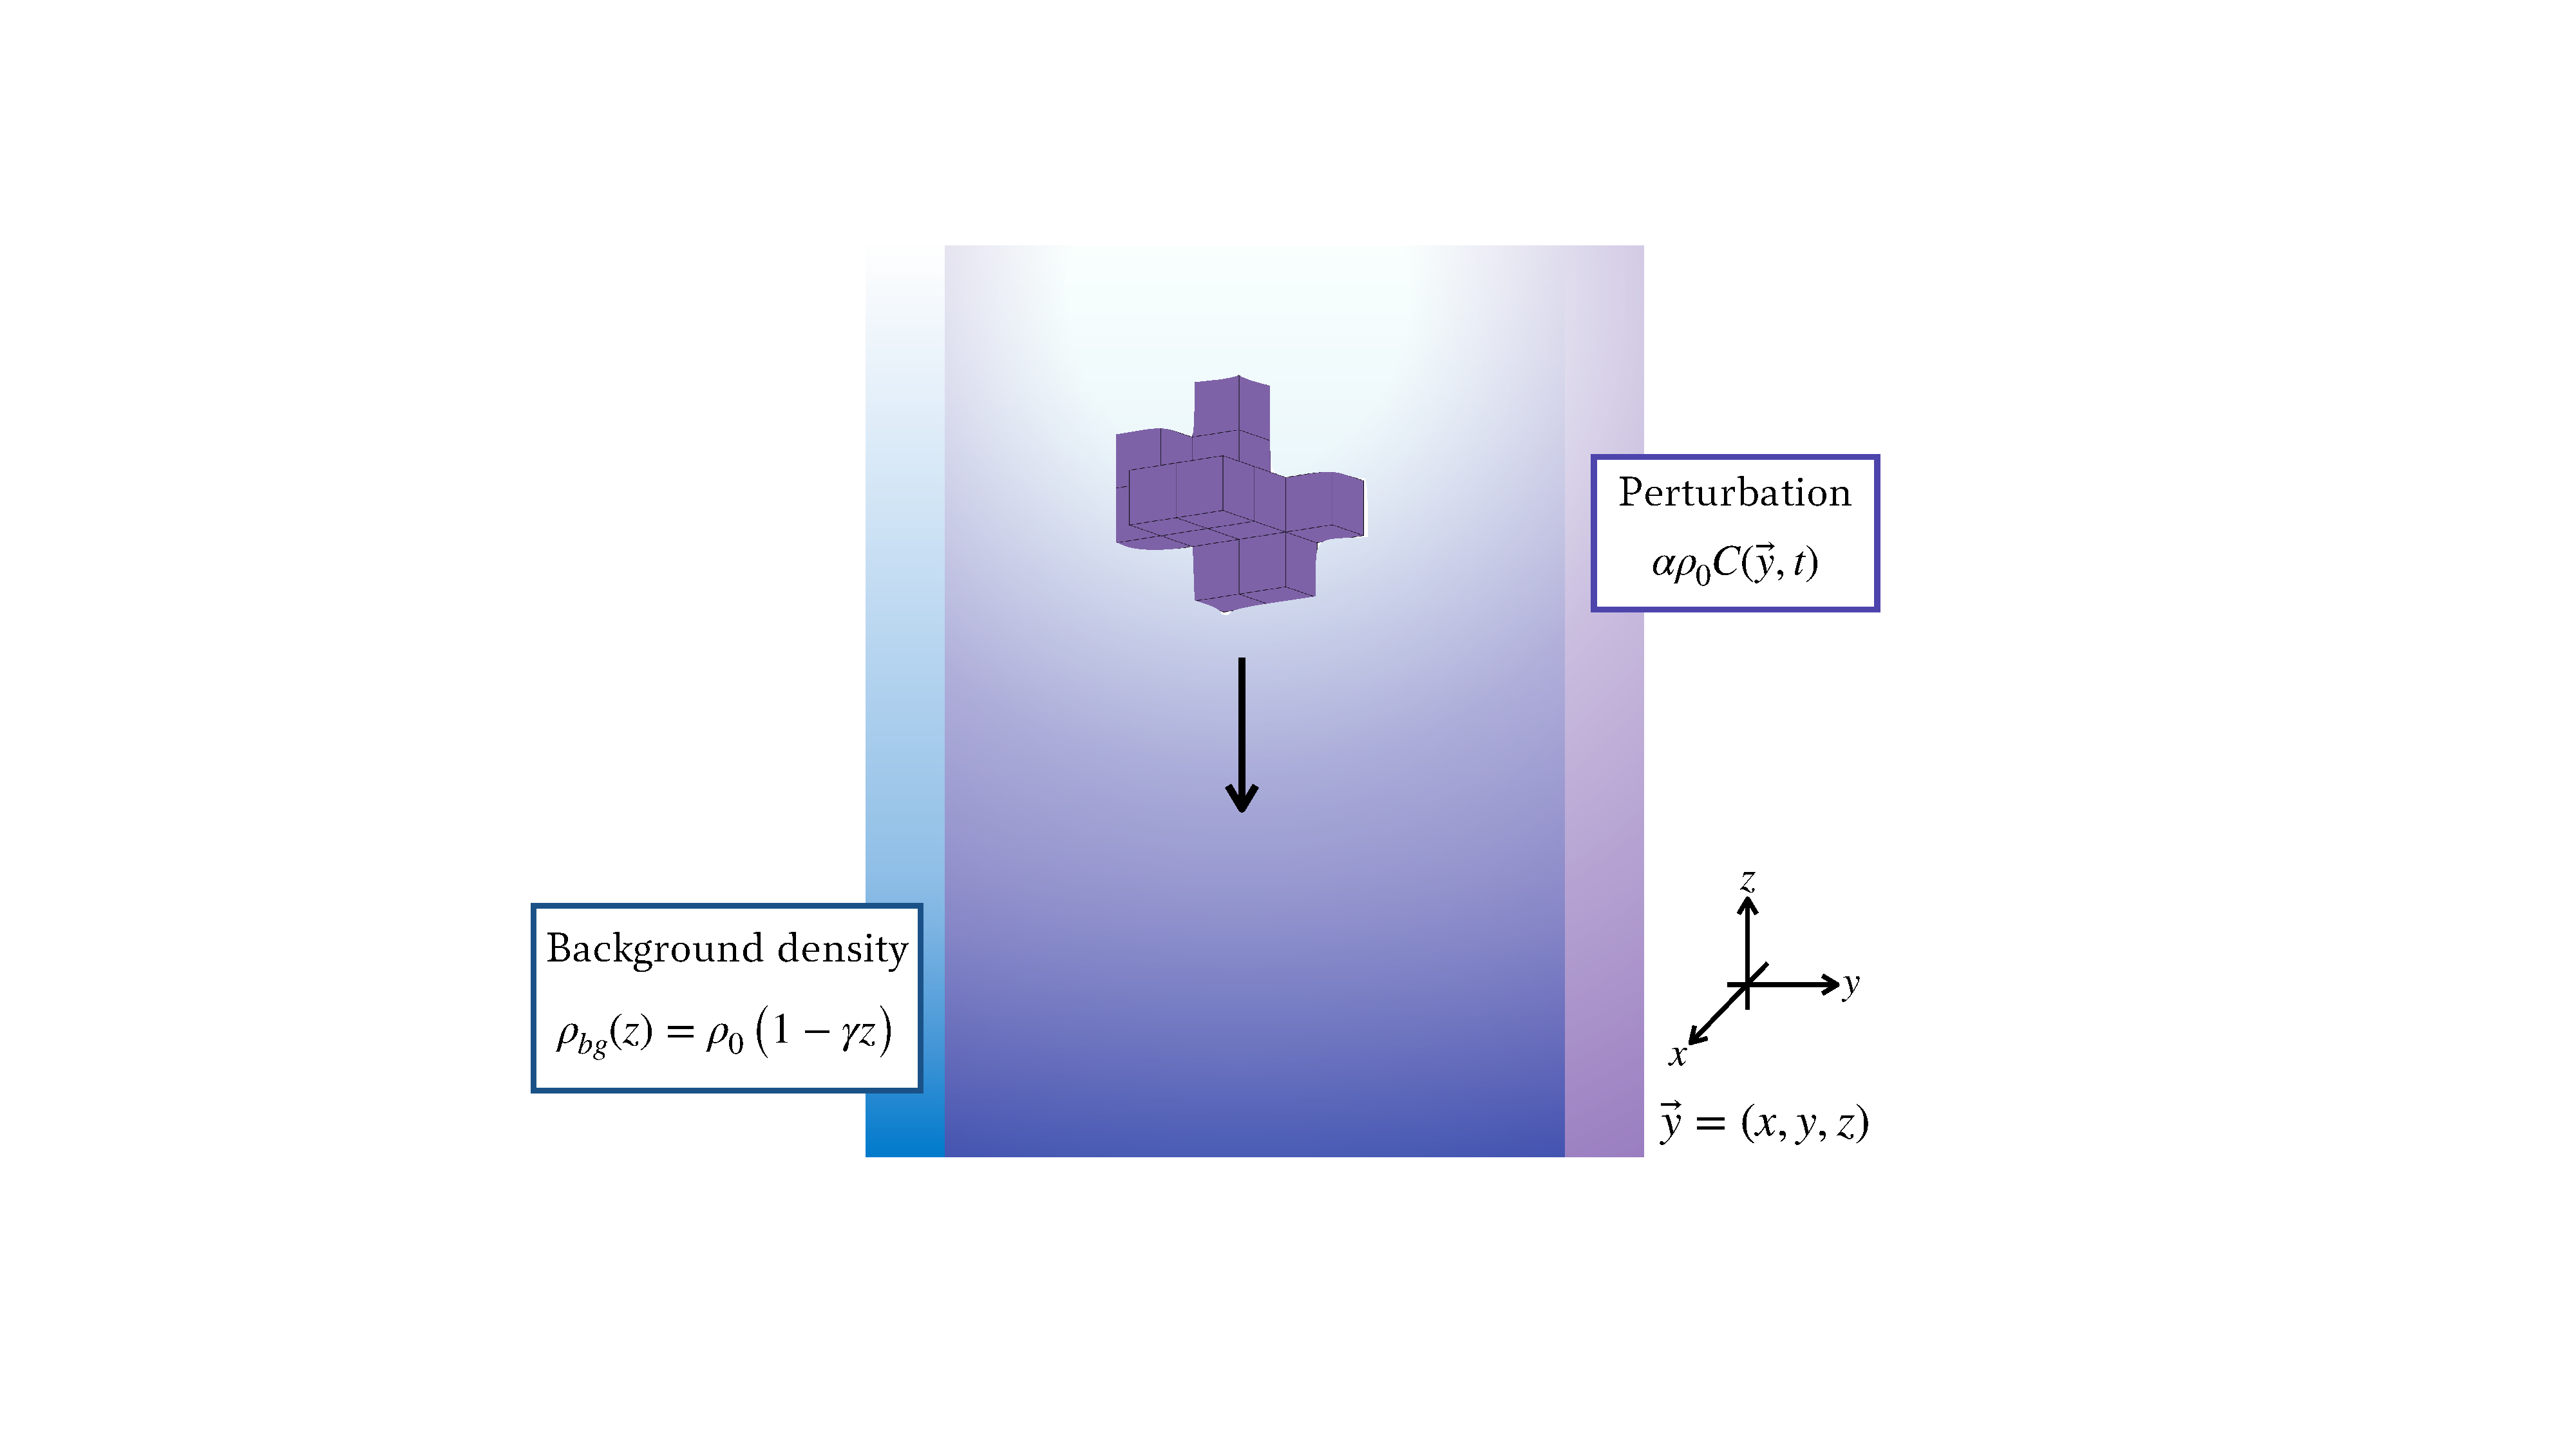
\includegraphics[scale=0.4]{./figures/fig_stratification_schematics}
	\caption{Description of fluid density stratification.}
	\label{fig_stratification_schematics}
	\end{center}
\end{figure}
To track the perturbation $C(\vec{y},t)$, we couple the advection-diffusion equation with the modified Stokes equations that we will describe in the next section. 
%------------------------------------------------------------------------------
\section{Governing Equations}
The non-constant density $\rho(\vec{y},t)$ plays a role as an external source of the fluid. This changes the momentum equation,
	Due to varying density, $\rho(\vec{y}, t)$, 
		 \begin{equation}
		\ \tilde{\mu}\nabla^2 \vec{u}(\vec{y})
		- \nabla P_d (\vec{y}) \ + \  
		 \rho_0 \alpha C(\vec{y},t) \vec{g} =0 , 
	\label{eq_extra_C}
	\end{equation}
	where $P_d$ is dynamic pressure, defined as
\begin{equation}
	P_d (\vec{y})
	 = P (\vec{y}) \ - \int \rho_{bg}(z) g   \textrm{d}z.
	\label{eq_Pd}
\end{equation}
To take the perturbation effect into account, we find the particular solution to the momentum equation (\ref{eq_extra_C}). Once we have one, simple addition to the homogenous solution would give us the entire solution due to the linearity of the system. 
\par
% \subsection{Particular solution to Stokes equations with the stratification}
%----------------------------------------------------------------------
To derive the particular solution, we consider the singularly forced Stokes problem \cite{pozrikidis_boundary_1992},
\begin{equation}
	\ \tilde{\mu} \nabla^2 \vec{u}(\vec{y})
	- \nabla P (\vec{y})
	+\vec{q} \ \delta \left(\vec{x} - \vec{y} \right) =0,
\label{eq_single_stokes}
\end{equation}
where $\vec{q}$ is an arbitrary constant vector, $\vec{y}$ is an arbitrary point in fluid domain, and $\delta$ is the three-dimensional delta function.
The problem (\ref{eq_single_stokes}) 
describes the effect coming from a single force applied at $\vec{x} = \vec{y}.$
The fundamental solutions to equation (\ref{eq_single_stokes}) with the continuity equation are
\begin{equation}
	\vec{u} (\vec{y}) = \ \frac{1}{8\pi \tilde{\mu}}  \bar{\bar{G \ }}(\vec{x}, \vec{y})
	\cdot  \vec{q}.
\label{eq_fund_u}
\end{equation}
\begin{equation}
	P (\vec{y}) = \ \frac{1}{4\pi }  
	\frac{\vec{x} - \vec{y}}{\| \vec{x} - \vec{y}\|^3}
	\cdot  \vec{q},
\label{eq_fund_p}
\end{equation}
where the kernel $\bar{\bar{G \ }}$ is called \textit{Stokeslet}, defined as 
\begin{equation}
	\bar{\bar{G}}( \vec{x}, \vec{y}) = 
	\frac{\bar{\bar{I \ }}}{||\vec{x}-\vec{y} ||} + \frac{(\vec{x}-\vec{y})(\vec{x}-\vec{y})^T}{||\vec{x}-\vec{y} ||^3}.
	% \label{eq_stokeslet_repeat}
\end{equation} 
This implies that the solutions (\ref{eq_fund_u}) and (\ref{eq_fund_p}) satisfy equation (\ref{eq_single_stokes}) as
\begin{equation}
	\ \tilde{\mu} \nabla^2 
	\biggl( \frac{1}{8\pi \tilde{\mu}}  \bar{\bar{G \ }}(\vec{x}, \vec{y})
	\cdot  \vec{q} \biggr)
	- \nabla \biggl(\ \frac{1}{4\pi }  
	\frac{\vec{x} - \vec{y}}{\| \vec{x} - \vec{y}\|^3}
	\cdot  \vec{q} \biggr)
	+ \vec{q} \ \delta \left(\vec{x} - \vec{y} \right)
	=0 .
\label{eq_single_stokes_sub}
\end{equation}
As we multiply by $\left( C(\vec{x}, t) \right)$ on both sides and integrate the entire equation over the domain, $V(\vec{x})$, we get
\begin{equation}
	\int_{V}
	\biggl[
	\ \tilde{\mu} \nabla^2 
	\biggl( \frac{1}{8\pi \tilde{\mu}}  \bar{\bar{G \ }}(\vec{x}, \vec{y})
	\cdot  \vec{q} \biggr)
	C(\vec{x}, t)
	-
	\nabla \biggl(\ \frac{1}{4\pi }  
	\frac{\vec{x} - \vec{y}}{\| \vec{x} - \vec{y}\|^3}
	\cdot  \vec{q} \biggr)
	C(\vec{x}, t)
	+ \vec{q} \ \delta \left(\vec{x} - \vec{y} \right)
	C(\vec{x}, t)
	\biggr]
	\ \textrm{d}V(\vec{x}) = 0 .
\label{eq_single_stokes_sub2}
\end{equation}

Note that the operator $\nabla$ is linear and used with respect to $\vec{x}$. We are able to switch the order with the integral operator as follows,
\begin{equation}
	\tilde{\mu} \ \nabla^2 
	\int_{V}
	\biggl( \frac{1}{8\pi \tilde{\mu}}  \bar{\bar{G \ }}(\vec{x}, \vec{y})
	\cdot  \vec{q} \biggr)
	C(\vec{x}, t)
	\ \textrm{d}V(\vec{x})
	-
	\nabla 
	\int_{V}
	\biggl(\ \frac{1}{4\pi }  
	\frac{\vec{x} - \vec{y}}{\| \vec{x} - \vec{y}\|^3}
	\cdot  \vec{q} \biggr)
	C(\vec{x}, t)
	\ \textrm{d}V(\vec{x})
	+\vec{q} C(\vec{x}, t) = 0 .
\label{eq_single_stokes_sub3}
\end{equation}
By choosing $\vec{q} = \rho_0 \alpha \vec{g}$, we can find the particular solutions to our modified Stokes equations, (\ref{eq_extra_C}),
\begin{equation}
	\vec{u} (\vec{y}) =
	 \frac{\rho_0 \alpha }{8\pi \tilde{\mu}}
	\int_{V}  \bar{\bar{G \ }}(\vec{x}, \vec{y})
	\cdot  C(\vec{x}, t) \vec{g} 
	\ \textrm{d}V(\vec{x}).
\label{eq_fund_soln_unit}
\end{equation}
\begin{equation}
	P(\vec{y}) = 
	\frac{\rho_0 \alpha }{4\pi }  
	\int_{V}
	\frac{\vec{x} - \vec{y}}{\| \vec{x} - \vec{y}\|^3}
	\cdot 
	C(\vec{x}, t) \vec{g} 
	\ \textrm{d}V(\vec{x}).
\label{eq_fund_soln_p}
\end{equation}
The entire velocity solution, thus, becomes
\begin{equation}
	 \vec{u} \left(\vec{y}, t \right) =
	 - \frac{1}{8 \pi \tilde{\mu}} \int_{S}  
		 \vec{f}(\vec{x}) 
		 \cdot \bar{\bar{G \ }} (\vec{x},\vec{y}) 
		 \ \textrm{d}S(\vec{x})
	+ \frac{ \rho_0 \alpha  }{8\pi \tilde{\mu}} \int_V  C \left(\vec{x},  t \right) \vec{g} \cdot 
	\bar{\bar{G \ }}(\vec{x}, \vec{y} ) 
	\ \text{d}V(\vec{x}).
\label{eq_vel_HP}
\end{equation}
As we see, the velocity at a point $\vec{u}$ is now depending on space and time. We can update the velocity field in time by coupling the solution (\ref{eq_vel_HP}) with the advection-diffusion equation. 
%------------------------------------------------------------------
\subsection{Force balance}
\label{sec:force_balance}
\par
We also want to point out that we can no longer impose the velocity of the aggregate since it is not physically valid.
This implies that the velocity on the aggregate, equation (\ref{eq_solidbody}), that is
\begin{equation}
	\vec{u}_s (\vec{x}, t)  = \vec{U}_a + \vec{\Omega} \times (\vec{x}- \vec{x}_{cm}),
	\nonumber
\end{equation}
becomes an unknown value. Specifically, we now need to solve for the translational and angular velocity, $\vec{U}_a$ and $\vec{\Omega}$, respectively, by prescribing the total body force and total torque. 
We can close the system since we have three vector equations for all unknowns. 
As we mentioned, to close the system of equations, we prescribe the following total drag force, $\vec{F}_o$, and torque, $\vec{Q}_o $,
\begin{equation}
	\int_S \vec{f} (\vec{x}) \ \textrm{d}S = \vec{F}_o
\label{eq_Fo}
\end{equation}
and
\begin{equation}
	\int_S \vec{f}\times (\vec{x} - \vec{x}_{cm}) \ \textrm{d}S = \vec{Q}_o = \vec{0}.
\label{eq_Qo}
\end{equation}
 Note that the drag force is induced by the dynamic pressure $P_d$ defined in equation (\ref{eq_Pd}). This implies that 
\begin{equation}
	\vec{F}_o 
	 = - \int_S \left[ 
	 - \left( P -  \int \rho_{bg}(z) g \ \textrm{d}z \right) \bar{\bar{I \ }} 
	 + \tilde{\mu} \left( \nabla \vec{u} + (\nabla \vec{u})^{T} \right)
	 \right] \cdot \hat{n} \ \textrm{d}S (\vec{y}).
\label{eq_Fo_Pd}
\end{equation}
As we observe the stress tensor inside of equation (\ref{eq_Fo_Pd}), 
\begin{equation}
	\bar{\bar{\sigma \ }} = 
 -  P  \bar{\bar{I \ }} 
 + \tilde{\mu} \left( \nabla \vec{u} + (\nabla \vec{u})^{T} \right).
\end{equation}
Thus, the full body force, $\vec{F}_g$, can be found in the following net force balance equation at equilibrium,
\begin{equation}
	\vec{F}_o (t)
	= - \vec{F}(t) - \vec{F}_b
	  = - \vec{F}_g(t)
	  -  \int_S \left( 
	   \int \rho_{bg}(z) g \ \textrm{d}z 
	 \right) \bar{\bar{I \ }}  \cdot
	\hat{n} \ \textrm{d}S (\vec{y}).
\label{eq_Full_Force}
\end{equation}
The last term, $\vec{F}_b$, in equation (\ref{eq_Full_Force}) represents buoyancy acting toward the aggregate. 
This gravitational force, $\vec{F}_g$, can also be interpreted as the gravitational force acting on the aggregate,
\begin{equation}
	% \vec{F} = (\rho_a - \rho)V_a\vec{g}
	\vec{F}(t) = \rho_a(t) V_a \vec{g}, 
\end{equation}
where $\rho_a$  and $V_a$ are the aggregate density and volume, respectively. 
% In addition to equation (\ref{eq_vel_HP}), we may use equations (\ref{eq_Full_Force}) and (\ref{eq_total_Torque_dlp}) to solve for velocity $\vec{u}(\vec{x}_s)$ and the unknown density, $\vec{\psi} \in [0, 1]$, on the aggregate.
%------------------------------------------------------------------
% \subsection{Aggregate density}
Marine aggregates are typically very porous, yet their permeability is low. To take the porosity, denoted as $\phi \in [0,1]$, into account, we define the density of an aggregate as 
\begin{equation}
	\rho_a (t) = \phi \rho_{f}(t) + (1-\phi) \rho_{s},
	\label{eq_rho_a}
\end{equation}
where $\rho_{f}$ and $\rho_s$ are the liquid and solid portion of the entire aggregate density, respectively. To obtain the liquid portion of the aggregate density, we take an average of fluid density where the aggregate locates $\rho_{f},$
\begin{equation}
	\rho_{f}(t) = \frac{1}{V_a}\int_{V_a} \rho(\vec{x}, t) \  \textrm{d}V(\vec{x}))
\end{equation}
We here consider the solid part of the aggregate density as $\rho_s \approx 1400 $kg$/$m$^3.$ 
We also set the porosity about $95\%$, or $\phi = 0.95$.

% I don't think the following belongs here:

%--------------------------------------------------
\subsection{Advection-Diffusion equation}
Since the perturbation $C(\vec{x}, t)$ is time-dependent, we couple the Stokes equations with the advection-diffusion equation to update $C(\vec{x}, t)$ in time. To take the background density into account, what we should update is the entire fluid density,
\begin{equation}
	\frac{\partial \rho(\vec{y},t)}{\partial t}
	+ \vec{u}(\vec{y}) \cdot \nabla \rho(\vec{y},t)
	 = D \nabla^2 \rho(\vec{y},t),
\label{eq_AD_rho}
\end{equation}
where $D$ is the diffusion coefficient.
For salinity of seawater, we find the diffusion coefficient, $D_{salt} = 2 \times 10^{-9}  (\text{m}^2\text{/s})$ from \text{\it Wollast and Garrels (1971)} \cite{wollast_diffusion_1971}. In addition, we recall the aggregate's settling speed ($U_s$), its maximum radius ($R_a$),
\begin{align}
	\text{Pe} 
	= \frac{U_s R_a }{D_{salt}} 
	\approx \frac{3.8 \times 10^{-4}(\text{m/s}) \times \left(5 \times 10^{-5} \right) (\text{m})}{2 \times 10^{-9} (\text{m}^2\text{/s})} = 9.5
\end{align}
\par 
For the thermal diffusivity, $D_{heat}$, we consider the value referred by {\it Nayar et. al (2016)} \cite{nayar_thermophysical_2016} and {\it Sharqawy et. al (2010)} \cite{sharqawy_thermophysical_2010},
\begin{align}
	\text{Pe} 
	= \frac{U_s R_a }{D_{heat}} 
	\approx \frac{3.8 \times 10^{-4}(\text{m/s}) \times \left(5 \times 10^{-5} \right) (\text{m})}{1.5 \times 10^{-7} (\text{m}^2\text{/s})} \approx 10^{-2}.
\end{align} 
Since the fluid density is evolving only in the gravitational direction, $z-$direction, we can simplify the re-write the equation (\ref{eq_AD_rho}) in terms of $C(z,t)$, 
\begin{equation}
	\frac{\partial C(z,t)}{\partial t}
	+ \vec{u}(\vec{y}) \cdot \nabla C(z,t)
	 = D \nabla^2 C(z,t)
	 + \frac{\gamma}{\alpha}\vec{u}(\vec{y})  \cdot \hat{k}.
\label{eq_AD_C}
\end{equation}
We track the perturbation $C(z,t)$ for every time step by solving the equation (\ref{eq_AD_C}).
%------------------------------------------------------------------
\section{Non-dimensionalization}
To facilitate further analysis, we non-dimensionalize our new equations. We mainly use the same parameters we introduced in section \ref{section3}, equations (\ref{eq_nonD}), in addition to the following dimensionless parameters:
\begin{equation}
	C= C_{max} C'
\hspace{7mm}
\rho = \frac{\tilde{\mu}  }{{U_s} R_a}  \rho', 
\end{equation}
In this chapter, the Stokes settling speed $U_s$, defined in equation (\ref{eq_U_s}), becomes
\[
U_s = \frac{g  L^2}{\tilde{\mu}}(\rho_s - \rho_0)(1-\phi),
\] 
since we consider the porosity of an aggregate as (\ref{eq_rho_a}).
% Note that the Reynolds number is approximately 0.03.
 % Here $\rho_a$ is the density of aggregate.
For the scale of the perturbation, $C$, we introduce the maximum density difference of the background density profile in the fluid domain at the initial time, i.e., 
\[
C_{max} = 
\left|
\max_{(x,y,z) \in V} \left(\rho_{bg}(z)  \right)
\ - \min_{(x,y,z) \in V} \left(\rho_{bg}(z)  \right) \right|.
 % \left| \tilde{S}(z_\text{top}, \ 0 )
 % - \tilde{S} \left( z_\text{bottom}, \ 0 \right) \right|. 
\] 
As we want to see the settling of an aggregate throughout the fluid having a density gradient, we decided to have 1\% density difference between the top and bottom layers of the fluid domain.
%  {\color{red}NEED NUMBER WITH UNIT AND A REFERENCE!}
\par
We first derived the dimensionless modified Stokes momentum equation,
\begin{equation}
	{\nabla'}^2  \vec{u}'(\vec{y})
	= \nabla {P_d}'(\vec{y}) \ - \  
	\frac{\rho_0}{(\rho_s - \rho_0)(1-\phi)} \alpha C_{max} C'\left(\vec{y},t \right)   \hat{k},
\label{eq_extra_C_nonD}
\end{equation}
along with the velocity field
%  on the aggregate boundary surface $\vec{y}' = \vec{x}'_s$, using 
 \begin{align}
		\vec{u}'(\vec{y})
			  & =- \frac{1}{8 \pi} \int_{S'}  
			 \vec{f'}(\vec{x}) 
			 \cdot \bar{\bar{G' \ }} (\vec{x},\vec{y}) 
			 \ \textrm{d}S'(\vec{x})
			 \nonumber \\
& -\frac{ \alpha C_{max}}{8\pi } \frac{\rho_0}{(\rho_s - \rho_0)(1-\phi)} 
\int_{V'} C' \left(\vec{x},  t \right) \hat{k} \cdot 
\bar{\bar{G'  }}(\vec{x}, \vec{y} ) 
\ \text{d}V'(\vec{x})
  \label{eq_vel_all_onS_nonD}
 \end{align}
where $S$ is the aggregate surface. 
Moreover, the force balance equation (\ref{eq_Full_Force}) becomes
\begin{align}
	 \vec{F'}_o(t)
	 & =
	   %\text{[Body force] + [Buoyancy force]}
	  %= 
	  \frac{1}{\tilde{\mu} U_s R_a} 
	  \left(
	-   \rho_a V_a g \hat{k}
	  +
	   \int_{S} \left( 
	   \int \rho_{bg}(z) g \ \textrm{d}z 
	   \right) \bar{\bar{I \ }}  \cdot
	  \hat{n} \ \textrm{d}S (\vec{x})
	\right).
\label{eq_Full_Force_nonD}
\end{align}

\par
Lastly, the advection-diffusion equation becomes, 
	\begin{equation}
	\frac{\partial C'(\vec{x},t)}{\partial t'}
	+ \vec{u}'(\vec{x}) \cdot \nabla' C'(\vec{x},t)
	 = \frac{1}{\textrm{Pe}} {\nabla'}^2 C'(\vec{x},t)
	 +\frac{\gamma R_a}{ \alpha C_{max}} \vec{u}' \cdot \hat{k},
	\label{eq_AD_nonD}
	\end{equation}
using the velocity field, equation (\ref{eq_vel_all_onS_nonD}), for the advection term.
For the rest of this chapter, we drop the prime for simplicity and use only dimensionless forms. 

%Rotation==============================================
\section{Rotation}
{\color{blue}QUESTION: MAYBE I SHOULD MOVE THIS SECTION TO NUMERICAL METHODS?}
To have more realistic simulations, we allow our aggregate model to rotate while they settle.
We here focus on the angular velocity, $\vec{\Omega} = \Delta \theta / \Delta t$, which tells us how much the aggregate rotates ($\theta)$ in one time step, $\Delta t$. 
\begin{figure}[ht]
	\begin{center}
		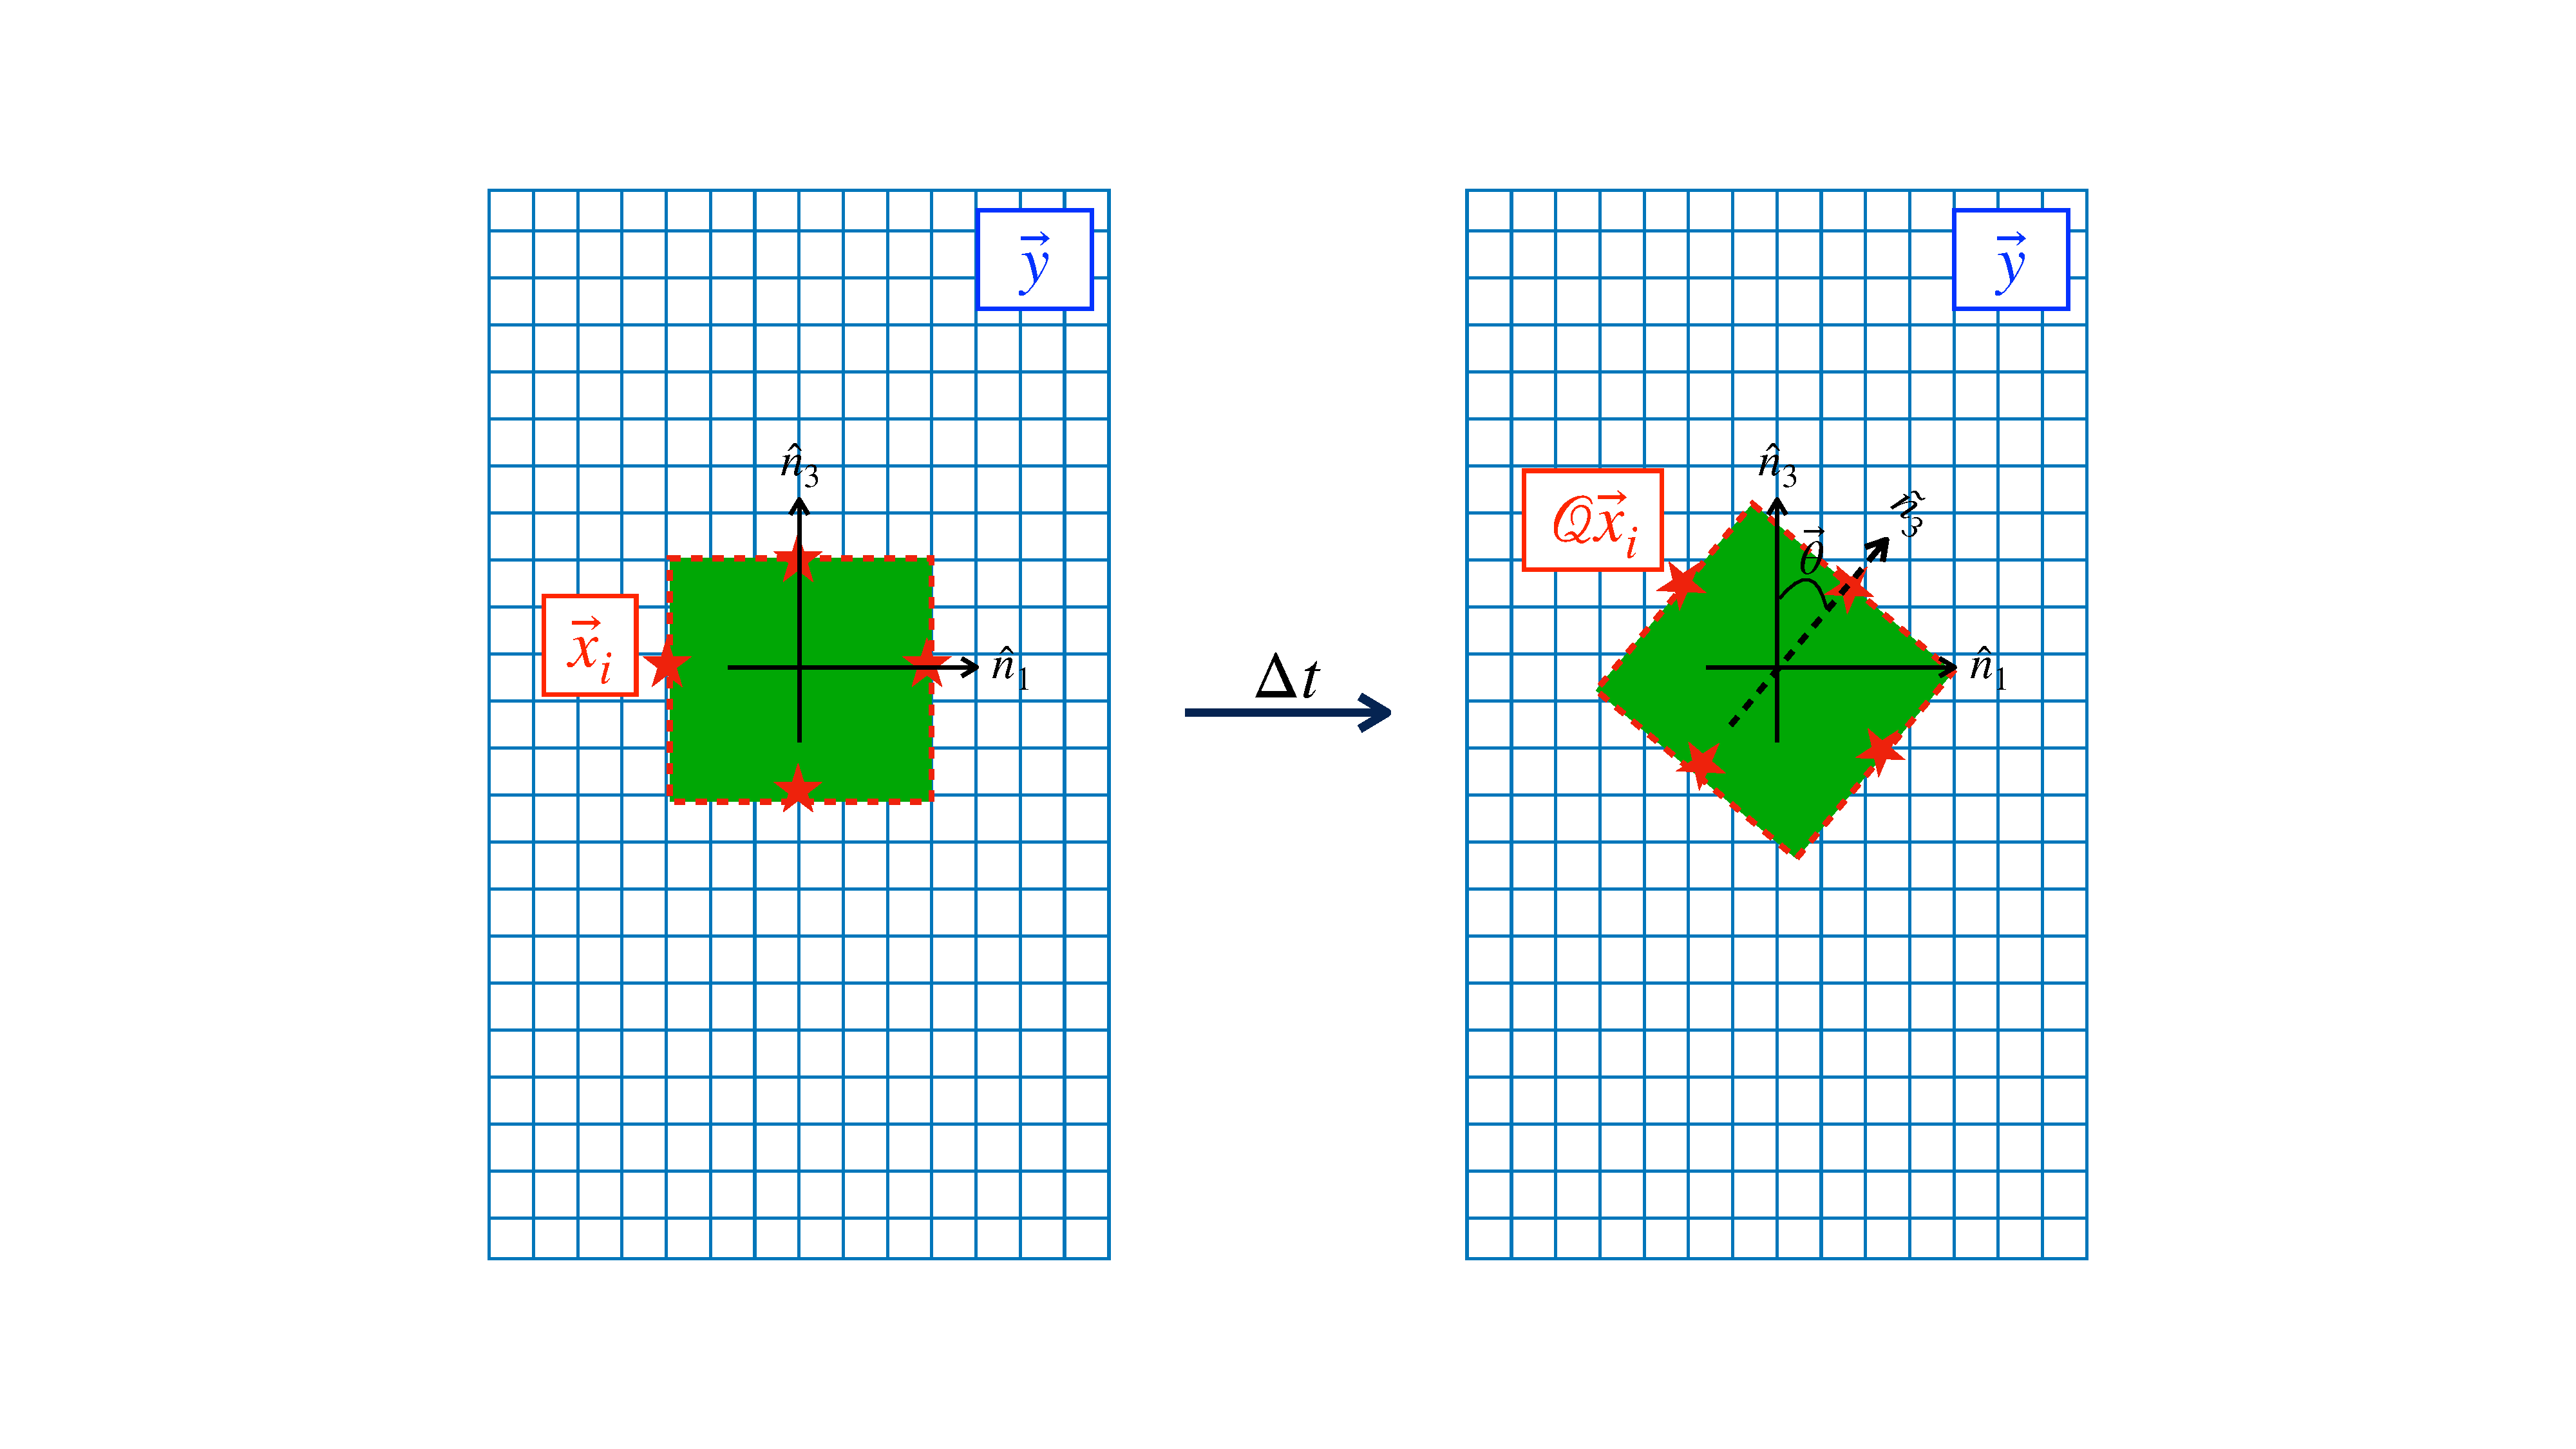
\includegraphics[scale=0.25]{./figures/fig_rotation_schematics.pdf}
	\caption{Schematics of the rotation of an aggregate. The blue grid is the fluid domain and the green rectangle represents an aggregate. Red stars show points on the aggregate.}
	\label{fig_rotation_schematics}
\end{center}
\end{figure}
This information lives in the orientation matrix, $\mathcal{Q}(t)$. We can update our aggregate position from $\vec{x}$ to $\vec{x}_{\mathcal{R}}$ using
\[
\vec{x}_{\mathcal{R}}(t) = \mathcal{Q}(t) \vec{x}.
\]
Note that $\mathcal{Q}(0) = \bar{\bar{I}}$ (identity matrix) at initial time. After we move forward one time step, we may update this orientation matrix as 
\begin{equation}
	\mathcal{Q}(t + \Delta t) = \mathcal{R} \mathcal{Q}(t),
\end{equation} 
where $\mathcal{R}$ is the rotation matrix. 
\par
Assume we obtain the angular velocity, $\vec{\Omega}$ from a time step. (Initially, it is zero vector). With this, we can find the three-dimensional change of angular position vector, $ \vec{\Omega} \Delta t = \left( \Delta \theta_1, \ \Delta \theta_2, \ \Delta \theta_3 \right) \equiv \Delta \vec{\theta}$.
The matrix $\mathcal{A}$ is then defined as 
\begin{equation}
	\mathcal{A}
	=\begin{bmatrix}
	 0 & - \Delta \theta_3 & \Delta \theta_2  \\
	 \Delta \theta_3 & 0  & -\Delta \theta_1  \\
	 - \Delta \theta_2 & \Delta \theta_1 & 0  \\
	\end{bmatrix},
	\label{eq_rotation_mx}
\end{equation}
From here, we have the rotation matrix $\mathcal{R} = e^{\mathcal{A}}.$
We can compute the matrix exponential $e^{\mathcal{A}}$ using Rodrigues' formula,
\begin{equation}
	\mathcal{R} = 
e^{\mathcal{A}} 
 = \bar{\bar{I \ }} 
 + \frac{\sin(\phi)}{\phi} \mathcal{A}
 + \frac{1-\cos(\phi)}{\phi^2} \mathcal{A}^2,
\label{eq_R_eA}
\end{equation} 
where $\phi = \|\Delta \vec{\theta}\|_2$.
With this $\mathcal{R}$ and orientation matrix $\mathcal{Q}$, we are ready to update the fluid grid.


	
\subsection{Linear system in a rotated coordinate}
We first solve for the stress at the center of each square face of an aggregate, $\vec{y} = \vec{x}_i$, 
using the same formula as equation (\ref{eq_vel_all_onS_nonD}),
\begin{equation}
	\vec{u} \left(\vec{x}_i \right) 
		  = -\int_{S}  
		 \vec{f}(\vec{x}) 
		 \cdot \bar{\bar{G \ }} (\vec{x}, \vec{x}_i) 
		 \ \textrm{d}S 
		 - \frac{ \alpha C_{max}}{8\pi } \frac{\rho_0}{(\rho_s - \rho_0)(1-\phi)}
		 \int_V  C \left(\vec{x} ,t \right) \hat{k} \cdot
		 \bar{\bar{G \ }}(\vec{x}, \vec{x}_i)
		 \ \text{d}V,
		 \nonumber
\end{equation}
As we allow rotation, we can express the above equation as
\begin{align}
	\vec{u} \left(\mathcal{Q} \vec{x}_i \right) 
		  = & - \frac{1}{8 \pi} \int_{S}  
		 \vec{f}(\mathcal{Q} \vec{x}) 
		 \cdot \bar{\bar{G \ }} (\mathcal{Q} \vec{x},\mathcal{Q}\vec{x}_i) 
		 \ \textrm{d}S
		 \nonumber \\
		 & - \frac{ \alpha C_{max}}{8\pi } \frac{\rho_0}{(\rho_s - \rho_0)(1-\phi)}
		 \int_V  C \left(\vec{x} ,t \right) \hat{k} \cdot
		 \bar{\bar{G \ }}(\vec{x}, \mathcal{Q} \vec{x}_i)
		 \ \text{d}V.
	\label{eq_slp_On_rotate}
\end{align}
Since the rotation matrix $Q$ is constant and it is normalized, it is valid to say that
\[
 \bar{\bar{G \ }} (\mathcal{Q} \vec{x},\mathcal{Q}\vec{x}_i) 
	 = \bar{\bar{G}}( \vec{x}, \vec{x}_i).
\]
We now solve for unknowns, including the translational and angular velocities,
in a rotated coordinate system $\mathcal{Q} \vec{x}_i $.
Note that the stress values we obtain here 
are located in the same one as the rotated positions.  
To complete the linear system to solve for stress, translational, and angular velocities, we temporarily map the fluid domain grid into the same coordinate system as the boundary integral term.
We can simply muptipliy by $\mathcal{Q}^{-1} = \mathcal{Q}^{T}$ as 
\begin{align}
	\vec{u} \left(\mathcal{Q} \vec{x}_i \right) 
		  & + \frac{1}{8 \pi} \int_{S}  
		 \vec{f}(\mathcal{Q} \vec{x}) 
		 \cdot \bar{\bar{G \ }} (\mathcal{Q} \vec{x},\mathcal{Q}\vec{x}_i) 
		 \ \textrm{d}S
		 \nonumber \\ & =
		 \mathcal{Q}^{-1}
		 \left[
		 - \frac{ \alpha C_{max}}{8\pi } \frac{\rho_0}{(\rho_s - \rho_0)(1-\phi)}
		 \int_V  C \left(\vec{x} ,t \right) \hat{k} \cdot
		 \bar{\bar{G \ }}(\vec{x}, \mathcal{Q} \vec{x}_i)
		 \ \text{d}V
		 \right].
	\label{eq_slp_vol_R}
\end{align}
For the other force equations as well, we implement the following
\begin{equation}
	\int_{S} \vec{f}(\vec{x}) \  \text{d}S(\vec{x})
	= \mathcal{Q}^{-1} \vec{F}_o
	 \label{eq_drag_code}
	 \end{equation} 
	 \begin{equation}
		 \int_S \vec{f} (\vec{x})  \times (\vec{x} - \vec{x}_{cm}) 
		 \ \textrm{d}S(\vec{x}) 
		 = \vec{0}.
	 \label{eq_torque_code}
	 \end{equation}
Once we solve the linear system, we may return the values on the fluid grid to the Cartesian coordinate system.
% We need to rotate them using
% \[
% \vec{f}(\vec{x}_s) = \mathcal{Q} \vec{f}(\vec{x}).	
% \]
% \[
% \vec{U}_a (\vec{x}_s) = \mathcal{Q} \vec{U}_a (\vec{x}).	
% \]
% \[
% \vec{\Omega}(\vec{x}_s) = \mathcal{Q} \vec{\Omega}(\vec{x}).	
% \]
% The validation of stress is in section (\ref{validation_rot}).
\subsection{Velocity compuation}
Once we solve for the stress, we are supposed to use the same 
equation (\ref{eq_vel_all_onS_nonD}) 
to solve for velocity in the fluid grid, which stays in the Cartesian coordinates.
Although the volume integral term can stay as it is,  
the boundary integral needs some special treatment
since it has two mixed coordinate systems.
We particularly pay more attention to the Stokeslet,
\[
	\bar{\bar{G \ }} (\mathcal{Q}\vec{x},\vec{y}) 
	= 
	\frac{\bar{\bar{I \ }}}{||\mathcal{Q}\vec{x}-\vec{y} ||} 
	+ \frac{(\mathcal{Q}\vec{x}-\vec{y})(\mathcal{Q}\vec{x}-\vec{y})^T}{||\mathcal{Q}\vec{x}-\vec{y} ||^3}, 	 
\]
where $\mathcal{Q}\vec{x}$ is in the aggregate rotated grid. Since we cannot compute the boundary integral of the Stokeslet when $\mathcal{Q}\vec{x}$ and $\vec{y}$ are not in the same coordinate system, we need to express $\vec{y}$ using another vector $\vec{v}$ that is in the rotated grid such that 
\[
	\mathcal{Q}\vec{x} - \vec{y} = \vec{x} - \vec{v},
	% \mathcal{Q}\vec{x}-\vec{v} = \vec{x} - \vec{y},
\]
or equivalently,
\[
	\vec{v} = \left(   \bar{\bar{I}} - \mathcal{Q} \right) \vec{x}  + \vec{y}.
\]
% {\color{blue} Need to type below figure.}
% \begin{figure}[h]
% 	\begin{center}
% 		\includegraphics[scale=0.45]{./figures/fig_vel_y_map}		
% 		\caption{Mapping for $\vec{y}$ grid.}
% 		\label{fig_vel_y_map}
% \end{center}
% \end{figure}

After we solve for the velocity field of the fluid domain, we rotate the velocity field back to the original coordinate by multiplying by the inverse of $\mathcal{Q}$ for the concentration update. 
%---------------Numerics--------------------------------------
\section{Numerical methods}
%-------------------------------------------------------------
In this section, 
We first consider aggregates drag computation. We derive the simplest form to implement in codes. We then revisit the velocity field calculation in a homogeneous fluid. We briefly introduce the linear system to solve for the aggregate's stress and velocity. Lastly, we present the method to compute the velocity field in a fluid with density, involving a volume integral of the perturbation $C(\vec{x},t)$. Due to the high computational cost, we use the fast multipole method (FMM). We briefly introduce the FMM and its framework for the Stokes kernel.
%subsection--------------------------------------------------------------------

\subsection{Aggregate force balance}
We first recall the force balance equation (\ref{eq_Full_Force}), introduced in section \ref{sec:force_balance}. To obtain the total drag, there are two types of forces we consider: 1) aggregate's body force, $\vec{F}_g$, and 2) fluid buoyancy force, $\vec{F}_b$. 
The aggregate density, $\rho_a$, of the fluid portion changes over time, which affects its (dimensionless) gravitational body force,
\begin{equation}
	\vec{F}_g = 
	- \frac{1}{\tilde{\mu} U_s R_a} 
	\left( \rho_a V_a g \hat{k}	 \right).
	\label{eq_agg_force_G}
\end{equation}
We also need to track the buoyancy, depending on the aggregate's vertical position,
\begin{align}
	\vec{F}_{b}
	 = \frac{1}{\tilde{\mu} U_s R_a} 
	 \left(
	  \int_{S} \left( 
	  \int \rho_{bg}(z) g \ \textrm{d}z 
	  \right) \bar{\bar{I \ }}  \cdot
	 \hat{n} \ \textrm{d}S (\vec{x})
   \right),
   \label{eq_buoyancy_nonD}
\end{align}
since the surrounding fluid density changes while the aggregate settles.
For further simplicity, we find an antiderivative of the background density,
\begin{equation}
	\mathcal{P}_{bg}(z) =  \int \rho_{bg}(z) g \ \textrm{d}z 
	 = \rho_0 \left( z - \frac{1}{2}\gamma z^2 \right) g,
\end{equation}
by choosing the lower bound of the integral as zero without loss of generality.
In practice, we can easily evaluate the gravitational force (\ref{eq_agg_force_G}). While settling, we compute the fluid density where the aggregate is located. Once we know which grid points are inside the aggregate, simply adding the densities at those points gives us the fluid density portion of the aggregate, which eventually plays a role in updating the $\rho_a$. 
\par
Next, we investigate the buoyancy force (\ref{eq_buoyancy_nonD}) with a single cube case for simplicity. 
We can extend this case to multiple cubes in the same manner by addition. We consider the discretized version of integral (\ref{eq_buoyancy_nonD}), 
\begin{equation}
	\vec{F}_b \approx
	\frac{1}{\tilde{\mu} U_s R_a} 
	\sum_{i=1}^{N_f}
	 R_a^3 \int_{S^i} 
	%  \left( 
		\mathcal{P}_{bg}(z) 
	%  \right) 
	 \bar{\bar{I \ }}  \cdot
	\hat{n}_i \ \textrm{d}S^i (\vec{x}),
\label{eq_buoyancy_discrete2}
\end{equation}
where $i$ represents the index of square faces (not power), and $N_f$ is the number of square faces: $N_f = 6$ for one cube case. Depending on the orientation of each square face, or the axis of $S^n$, is different. For example, let $S^1$ be the first square with the normal $\hat{n}_1 = (1,0,0)$, and surface parametrized with $y$ and $z$ between $-1$ and $1$,
\begin{align}
	\mathcal{L}_1 \equiv 
	R_a^3 
	 \int_{S^1}
	 \mathcal{P}_{bg}(z) 
	  \bar{\bar{I \ }}  \cdot
	\hat{n}_1 \ \textrm{d}S^1 (\vec{x})
	= R_a^3  \int_{-1}^{1} \int_{-1}^{1}
	\mathcal{P}_{bg}(z) 
	\bar{\bar{I \ }}  \cdot
 	\hat{n}_1 \ 
	\textrm{d}y  \textrm{d}z.
\label{eq_buoyancy_S1_2}
\end{align}
See Figure \ref{fig_rho_bg_on_S1} for notations.
\begin{figure}[h]
	\begin{center}
		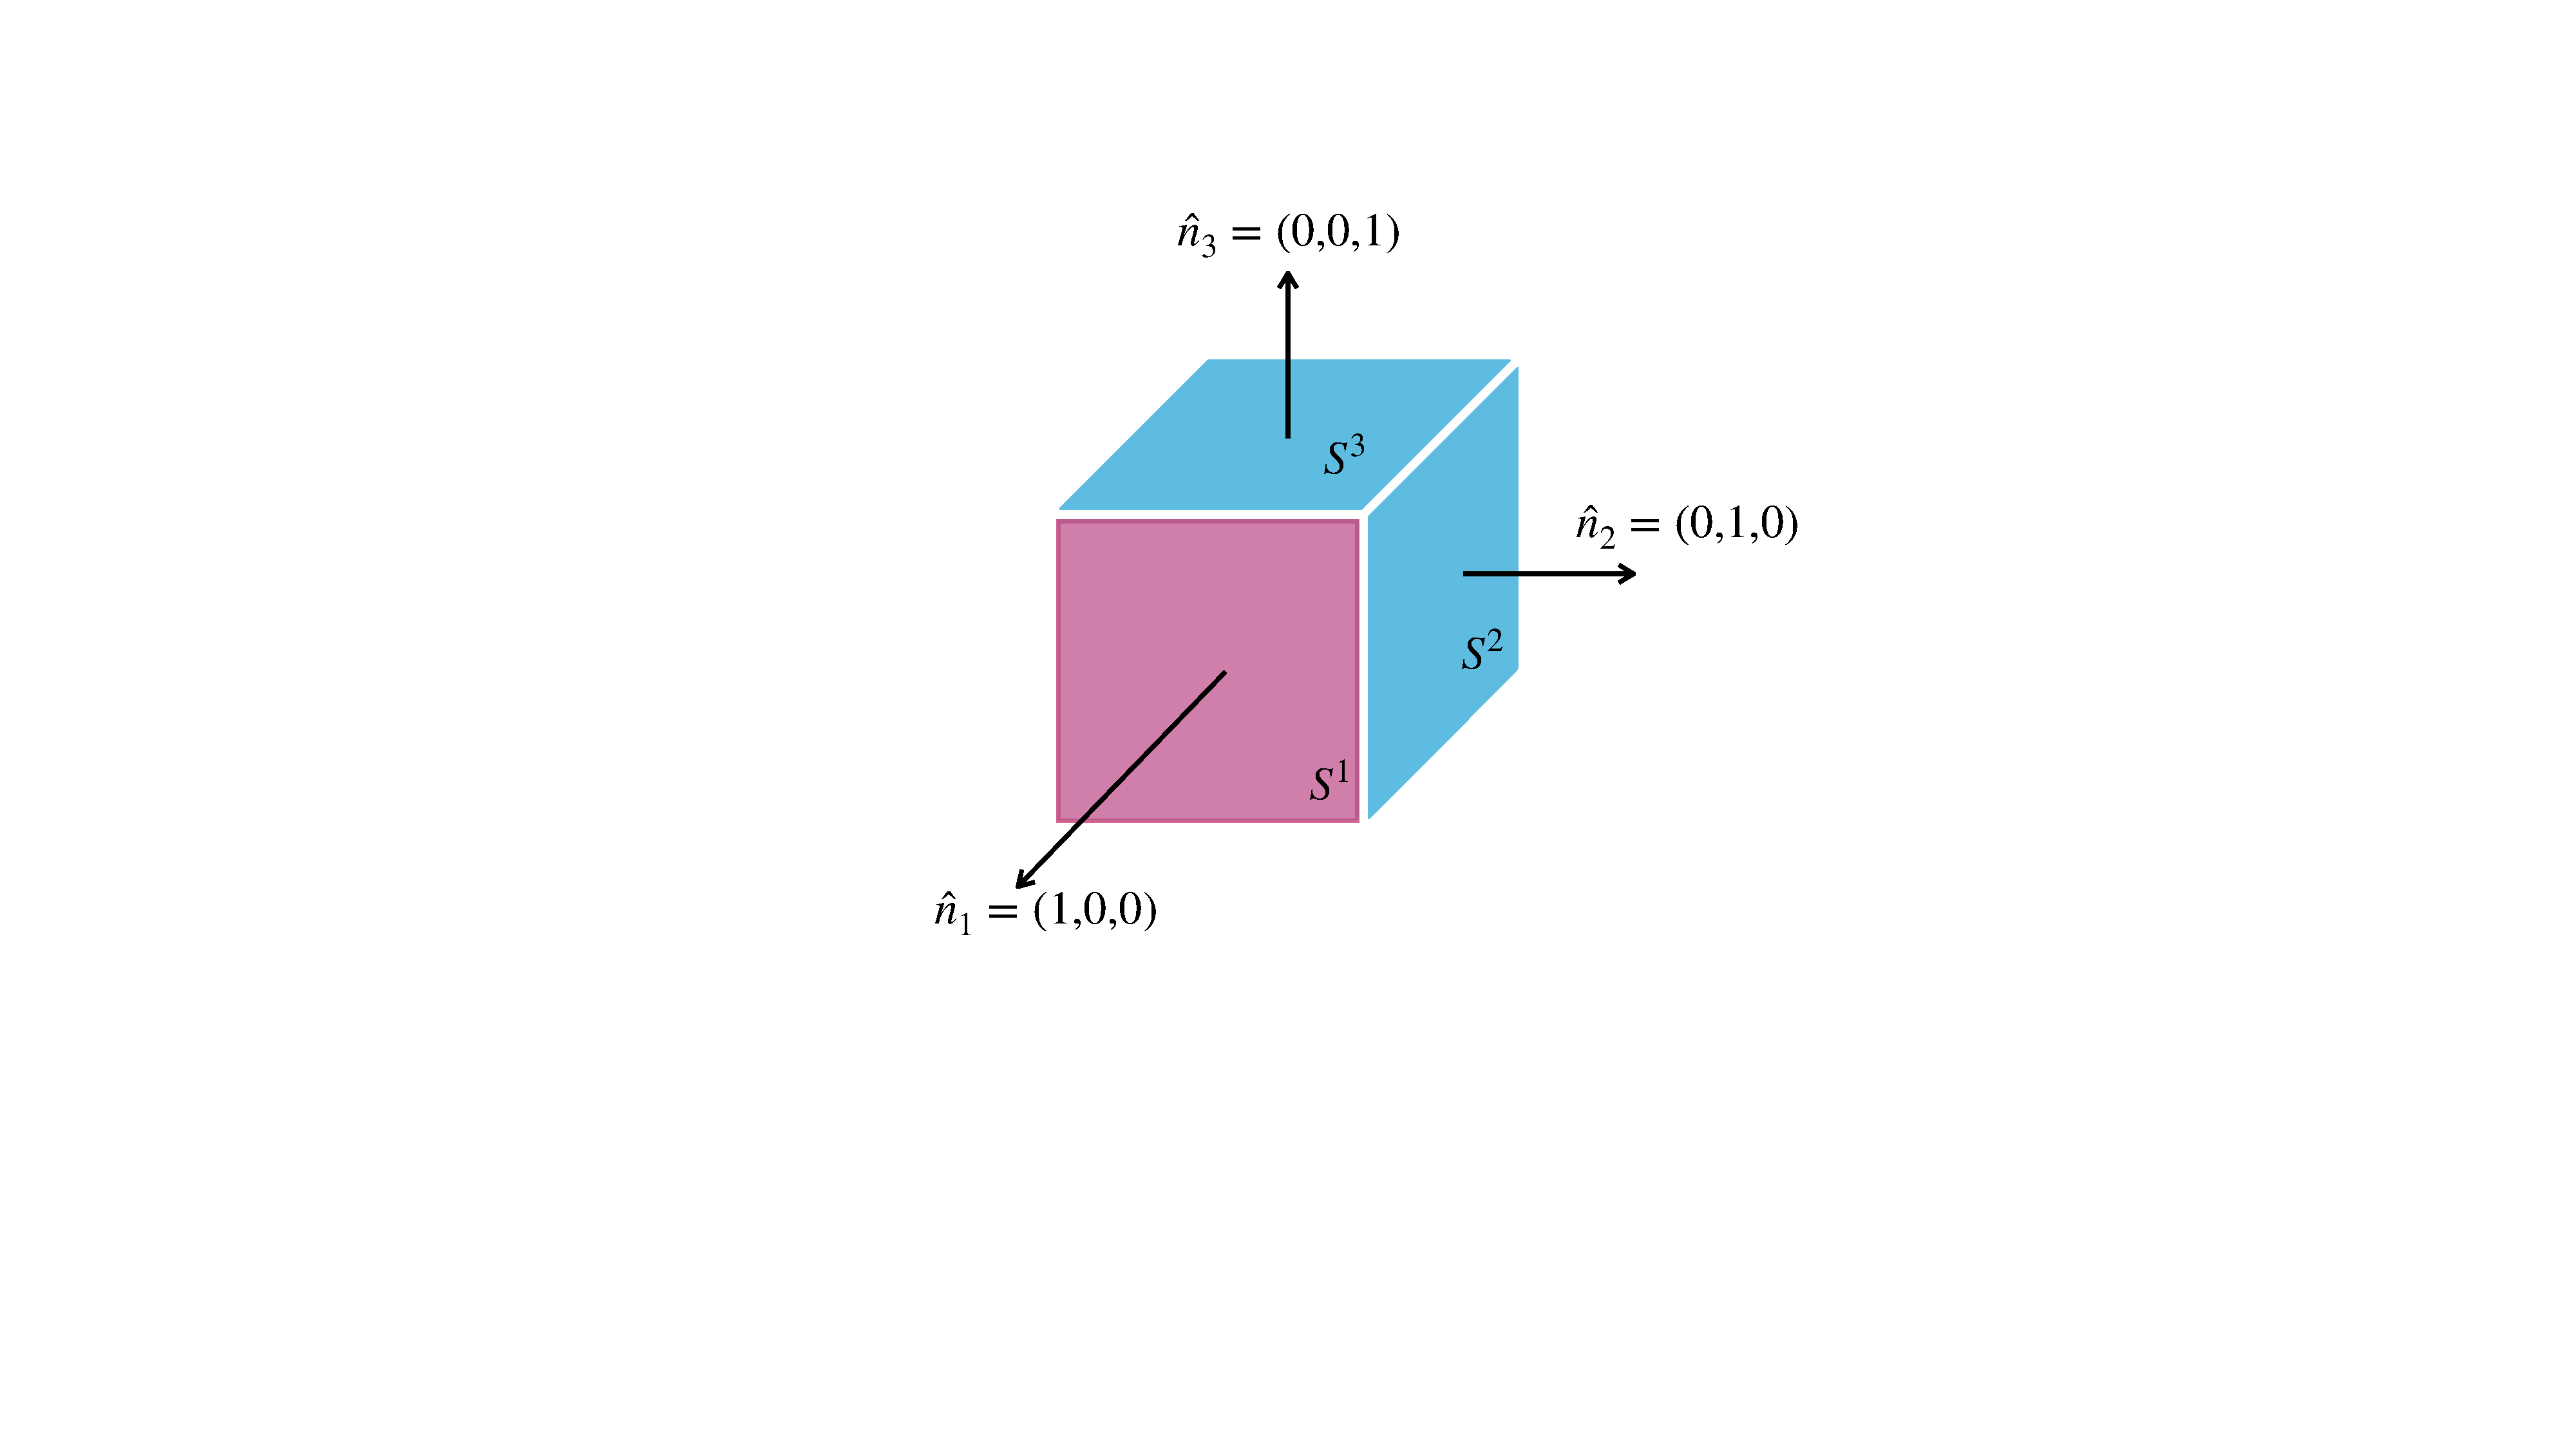
\includegraphics[scale=0.3]{./figures/fig_rho_bg_on_S1.pdf}
	\caption{Example cube to describe the buoyancy force computation. The pink area is $S^1$ integral domain.}
	\label{fig_rho_bg_on_S1}
\end{center}
\end{figure}
Since the background density $\rho_{bg}$ is a function of $z$-axis only, we can intuitively see that the value (\ref{eq_buoyancy_S1_2}) and the one with the normal $\hat{n}_6 = -\hat{n}_1 = (-1,0,0)$ has the same magnitude but in the opposite direction, and thus, we have $\mathcal{L}_6 = -\mathcal{L}_1$. 
It implies the following.
\begin{equation}
	\sum_{i=1,2,5,6}
	 R_a^3 \int_{S^i} 
	 \mathcal{P}_{bg}(z) 
	 \bar{\bar{I \ }}  \cdot
	\hat{n}_i \ \textrm{d}S^i (\vec{x})
	 = 0
\label{eq_buoyancy_zero_oneCube}
\end{equation}
for the one cube case of discretized buoyancy equation (\ref{eq_buoyancy_discrete2}).
\par
The integrals on $S^3$ and $S^4$ are slightly different since the square faces are perpendicular to $z-$axis. On the face $S^3$, which has normal $\hat{n}_3 = (0,0,1)$, we get
\begin{equation}
	R_a^3
\rho_0\int_{-1}^{1} \int_{-1}^{1}
  	\left( 
  	 z - \frac{\gamma}{2}{z}^2 
 	\right)g  \bar{\bar{I \ }}  \cdot
 	\hat{n}_3 \ 
	\textrm{d}x  \textrm{d}y 
	= 4 R_a^3 \rho_0 \left( z_T - \frac{\gamma}{2} {z_T}^{2} \right) g \hat{n}_3,
	\label{eq_F_by_S3}
\end{equation} 
where $z_T$ is the constant $z-$level value on the face $S^3$. The integral value on the face $S^4$ would be the same as (\ref{eq_F_by_S3}), having $\hat{n}_4 = (0,0,-1)$ instead of $\hat{n}_3$. We then can have a more explicit expression for the discretized buoyancy equation (\ref{eq_buoyancy_discrete2}),
\begin{align}
	& \sum_{i=1}^{6} R_a^3
	 \int_{S^i}
	 \mathcal{P}_{bg}(z) 
	  g \bar{\bar{I \ }}  \cdot
	\hat{n}_i \ \textrm{d}S^i (\vec{x})
	\nonumber 
	\\
	& = 4 R_a^3 \rho_0 \left( z_T - \frac{\gamma}{2} {z_T}^{2}  \right) g \hat{n}_3
	+ 4R_a^3 \rho_0 \left( z_B - \frac{\gamma}{2} {z_B}^{2}  \right) g \hat{n}_4,
\label{eq_buoyancy_discrete_eval2}
\end{align}
where $z_B$ is the constant $z-$ value of the surface $S^4$ (bottom face). By substituting the normals $\hat{n}_3$ and $\hat{n}_4$, we can simplify the right-hand side of equation (\ref{eq_buoyancy_discrete_eval2}), knowing that $z_T - z_B = 2$, the equation (\ref{eq_buoyancy_discrete_eval2}) becomes 
\begin{equation}
	\sum_{i=1}^{6} R_a^3
	\int_{S^i} 
	\mathcal{P}_{bg}(z) 
	g \bar{\bar{I \ }}  \cdot
   \hat{n}_i \ \textrm{d}S^i (\vec{x})
= 8 R_a^3 \rho_0 \left( 1 - \gamma z_{c_n} \right) g, 
\label{eq_buoyancy_z_eval2}
\end{equation}
where we define the $z-$component of the center of $n-$th cube forming an aggregate, $z_{c_n}$ ($ n = 1, 2, \cdots, NC$).
We thus have shown that the only information we need to keep track of is the location of the center of each cube that forms an aggregate.
%
 \subsection{Linear system for velocity and stress on aggregates}
As mentioned in section \ref{sec:force_balance}, we do not prescribe the settling velocity of an aggregate, and it becomes one of our unknowns.
We thus need to solve for 1) translational velocity ($\vec{U}_a$), 2) rotational velocity ($\vec{\Omega}$), and 3) stress vector ($\vec{f}_k$) on each square face $k$.
% To do so, we build a linear system using equations (\ref{eq_Fo}), (\ref{eq_Qo}). 
To do so, for any point $\vec{y}$ on the surface of the aggregate, we consider the surface velocity equations (\ref{eq_vel_all_onS_nonD}) with the solid body motion, (\ref{eq_solidbody}), 
 \begin{align}
	\vec{U}_a + \vec{\Omega} \times (\vec{y} - \vec{x}_{cm})
+ \frac{1}{8 \pi} \int_{S}  
		  \vec{f}(\vec{x}) 
		  \cdot \bar{\bar{G  }} (\vec{x},\vec{y}) 
		  \ \textrm{d}S(\vec{x})
		  \nonumber \\
=  -\frac{ \alpha C_{max}}{8\pi } \frac{\rho_0}{(\rho_s - \rho_0)(1-\phi)} 
\int_{V} C\left(\vec{x},  t \right) \hat{k} \cdot 
\bar{\bar{G}}(\vec{x}, \vec{y} ) 
\ \text{d}V(\vec{x}),
 \label{eq_slp_lin_eq}
 \end{align}
where the volume integral value on the right-hand side is known. 
To set up the linear system accordingly, We discretize the boundary integral as described in equation (\ref{eq_discretized}), choosing $\vec{f}_k$ for $\vec{q}_k$, and $ \bar{\bar{G}}$ for $\bar{\bar{J}}$, 
\begin{equation}
	\vec{I}(\vec{x}_{sq,i})  =   \sum_{k=1}^{N_f}  \vec{f}_k   \int_{S_{k}} \bar{\bar{G}}(\vec{x},\vec{x}_{sq,i}) \ \text{d}S(\vec{x}) 
	= \sum_{k=1}^{N_f} \vec{f}_k   \ \bar{\bar{\Pi}}_{i,k}
	\approx \int_{S}  
	\vec{f}(\vec{x}) 
	\cdot \bar{\bar{G  }} (\vec{x},\vec{x}_{sq,i}) 
	\ \textrm{d}S(\vec{x}),
\end{equation}
where $\vec{x}_{sq, i}$ is the center of each square on the surface for $i = 1, \  2, \cdots, \  N_f$.
With equations (\ref{eq_Fo}), (\ref{eq_Qo}), the exact linear system of the equations we implement is as follows.
 \begin{align}
	\tiny
		%---A------------------------------------------------------------
 	\left[
 	    \begin{array}{c;{2pt/2pt}c; {2pt/2pt}c}
 			\phantom{,} & \phantom{,}& \phantom{,}
 			\\
		   \begin{bmatrix}
 				\bar{\bar{\Pi}}_{1,1} & 
 				\bar{\bar{\Pi}}_{1,2} &
 				\cdots & \bar{\bar{\Pi}}_{1,N_f}
 				\\
 				\\
 				\bar{\bar{\Pi}}_{2,1} & 
 				\bar{\bar{\Pi}}_{2,2} &
 				\cdots & \bar{\bar{\Pi}}_{2,N_f}
 				\\ 
 				\vdots &  \vdots & \ddots & \vdots
 				\\
 				\\
 				\bar{\bar{\Pi}}_{N_f,1}&
 				\bar{\bar{\Pi}}_{N_f,2} &
 				 \cdots & \bar{\bar{\Pi}}_{N_f,N_f}
 		\end{bmatrix}
 			 & 
 			 \begin{bmatrix}
 				 \bar{\bar{I \ }}
 				 \\
 				 \vdots
 				 \\
 				 \\
 				  \bar{\bar{I \ }}
 			\end{bmatrix}
 			  & -
    			 \begin{bmatrix}
    				  [\vec{x}_{sq,1} - \vec{x}_{cm}]_{\times}
    				 \\
    				 \vdots
    				 \\
    				 \\
    				   [\vec{x}_{sq,N_f} - \vec{x}_{cm}]_{\times}
    			\end{bmatrix}
 			\\
 			\phantom{,} &\phantom{,} &\phantom{,}
 			\\
 			\hdashline[2pt/2pt]
 			\phantom{,} &\phantom{,} &\phantom{,}
 			\\
 			 4 \begin{bmatrix}
 				  \bar{\bar{I \ }}
 				 &
 				 \cdots
 				 &
 				  \bar{\bar{I \ }}
 			\end{bmatrix}
 			&  \bar{\bar{0}}  & \bar{\bar{0}}
 			\\
 			\phantom{,} &\phantom{,} &\phantom{,}
 			\\
 			 \hdashline[2pt/2pt]
 			 \phantom{,} &\phantom{,} &\phantom{,}
 			\\
 			 - 4 \begin{bmatrix}
 				[\vec{x}_{sq,1} - \vec{x}_{cm}]_{\times}
 				 &
 				 \cdots
 				 &
 				  [\vec{x}_{sq,N_f} - \vec{x}_{cm}]_{\times}
 			\end{bmatrix}
 			& \bar{\bar{0}}  &  \bar{\bar{0}}
  	 	\\
 			\phantom{,} & \phantom{,}& \phantom{,}
 	    \end{array}
 	\right]
 	%---x------------------------------------------------------------
 	\left[
 	\begin{array}{c}
 		\vec{f}_1
 		\\ \\
 		\vdots \\
 		\\
 		\vec{f}_{N_f}
 		 \\ \\  \hdashline[2pt/2pt]
 		\\
 		 \vec{U}_a
 	  	\\
 	 	\\
 	 	\hdashline[2pt/2pt]
 	 	\\
 	 	\vec{\Omega}
 	\end{array}
 	\right]
 		%---b------------------------------------------------------------
 	=
 	\left[
 	\begin{array}{c}
 		{\vec{\mathcal{F}}}^1  \\ \\
 		\vdots \\
 		\\
 		{\vec{\mathcal{F}}}^{N_f} \\ \\  \hdashline[2pt/2pt]
 		\\
 		 \vec{F}_o
 	  	\\
 	 	\\
 	 	\hdashline[2pt/2pt]
 	 	\\
 	 	\vec{Q}_o
 	\end{array}
 	\right].
 \label{eq_slp_linear_system}
 \end{align}
 Since we consider three-dimensional space, the size of the identity matrix $\bar{\bar{I}}$ is $(3 \times 3)$. The matrix $[\vec{y}]_{\times}$ represents the cross product operator defined by,
 \begin{equation}
 	[\vec{y}]_{\times} = \begin{bmatrix}
 	0 & -y_3  & y_2 \\ 
 	 y_3 & 0  & -y_1\\ 
 	- y_2 & y_1  & 0
 	\end{bmatrix},
 	\label{eq_cross_2}
 \end{equation}
 where $\vec{y} = (y_1, y_2, y_3).$
We use this operator for the rotation term, 
 \[
  [\vec{x} - \vec{x}_{cm}]_{\times}  \vec{\Omega}
   = (\vec{x} - \vec{x}_{cm}) \times \vec{\Omega}
  = - \vec{\Omega} \times  (\vec{x} - \vec{x}_{cm}),
  \]
in the total torque equation.
In addition, the top part of the right-hand side of equation (\ref{eq_slp_lin_eq}) is the discretization of the volume integral,
\begin{equation}
	{\vec{\mathcal{F}}} (\vec{x}_{sq,i}) = 
	-\frac{ \alpha C_{max}}{8\pi } \frac{\rho_0}{(\rho_s - \rho_0)(1-\phi)} 
   \sum_{j= 1}^{Ns}  C \left(\vec{x}_{sq,i},  t \right) \hat{k} \cdot
   \bar{\bar{G \ }}(\vec{x}_{sq, i}, \vec{x}_{j} ),
\label{eq_volume_rhs}
\end{equation}
   where $N_s$ is the total number of grid or source points in the fluid domain. We discuss more details of the volume integral computation in the next section. 
%    \ref{section_volume_int}.
  One can find factor 4 multiplied by the second and third blocks on the right-hand side of the system (\ref{eq_slp_linear_system}). 
 Since we set the side length of a cube as 2, factor 4 represents the area of a square face that is the integral domain of the total force and torque equations. 
 \par
 Once we solve the linear system and obtain the unknowns, we use the equation (\ref{eq_vel_all_onS_nonD}) to calculate the velocity field at all points in the fluid domain. We want to point out that the fluid velocity computation, especially including the volume integral (\ref{eq_volume_rhs}), is a very numerically expensive calculation. To accelerate it, we apply the fast multipole method (FMM) to our simulations. In the following section, we explain how we use the FMM. 
 %
 %
 %----FMM--------------------------------------------------------------------------
\subsection{Fast Multipole Method (FMM)}
Knowing that we simulate our problem in a three-dimensional fluid domain, it is necessary to implement an efficient and fast method for each part of the codes while we keep the stability and desired accuracy. 
The FMM is a numerical scheme for rapid computation of $N$-body problems governed by a Green's function using a multipole expansion. It was first introduced by Greengard and Rokhlin \cite{greengard_fast_1987}. Since then, the researchers at Flatiron Institute - Simons Foundation,  including the original authors of the FMM, have developed the methods and shared the source code. \cite{cheng_fast_1999,greengard_new_1997,greengard_new_2002} We choose to use their library, called \href{https://github.com/flatironinstitute/FMM3D}{{\color{blue}FMM3D}}. It provides the code of the $N-$body interactions governed by Laplace and Helmholtz equations in three-dimension.
For our problem, we can modify the Laplace kernel, as shown in \cite{tornberg_fast_2008}, to compute the integrals of Stokeslet (\ref{eq_stokeslet}).
The definition of Laplace FMM in the FMM3D library is the following:
\begin{definition} (\textit{Laplace FMM})
	\label{eq_def_FMM}
	Let $c^n \in \mathbb{R}$ denote a collection of charge strengths and $\vec{v}^n \in \mathbb{R}^3$ denote a collection of dipole strengths for $n = 1,2, \cdots, N$.
	The Laplace FMM computes the potential $u(\vec{y}^m) \in \mathbb{R}^3$ given by
\begin{equation}
	u(\vec{y}^m) = \sum_{n = 1}^{N} 
		\Biggl[
		\frac{c^n}{\|\vec{x}^n - \vec{y}^m \|}
			- \vec{v}^n \cdot \nabla_{\vec{y}} 
			 \frac{1}{\|\vec{x}^n - \vec{y}^m \|}
		\Biggr],
\label{eq_fmm3d_package}
\end{equation}
	at the \textit{source} ($\vec{x}^n$) and \textit{target} locations ($\vec{y}^m$). 
	% Here, the denominator $\|x_i^n - y_j^m \| = \|\vec{x}^n - \vec{y}^m \|$.
	When $\vec{y}^m = \vec{x}^n$, the term corresponding to $\vec{x}^n$
	is dropped from the sum.
\end{definition}
\noindent
Note that we use the letters $m$ and $n$ to index the targets and sources, respectively. For our problem, the points where we want to obtain velocity would be the targets; all points in an integral domain are sources.
In addition to the target and source points, we can input the constant $c^n$ and vector $\vec{v}^{n}$. One needs to be careful about these terms; both values could depend on the sources but are independent of the targets. 
\subsubsection{Volume integral of the Stokeslet}
We first investigate how to incorporate the volume integral (\ref{eq_volume_rhs}) (without the prefactor) in the form of (\ref{eq_fmm3d_package}). For a fixed $j$, we can rewrite the equation using the index notation ($i, j = 1,2,3$), 
\begin{equation}
	\tilde{V}(y_j^m)
	\equiv
	 d\sum_{n = 1}^{Ns} \sum_{i = 1}^{3}
	 C(x^n_i,  t)\hat{k} G_{ij}(x_i^n,y_j^m),
	\label{eq_Vn}
\end{equation}
where $\vec{y}^m = (y_1^m, \ y_2^m, \ y_3^m)$ is the target point, $\vec{x}^n = (x_1^n, \ x_2^n, \ x_3^n)$ are the source or grid points in the fluid domain $V$, and $d$ is constant from a quadrature method.
Note that we can use the FMM3D only for points $\vec{y}^m \neq \vec{x}^n \in V$. 
At a singularity, i.e.,  $\vec{y}^m = \vec{x}^n $, we use MATLAB built-in function, \verb+integral3+, to integrate numerically by defining a small cube $V_p$ around the singularity point,
\begin{equation}
	\mathbb{V}_p(\vec{y}) = 
	 \int_{{V}_p}
		C (\vec{x},t ) \hat{k} \cdot 
		\bar{\bar{G \ }} (\vec{x}, \vec{y} ) 
		\ \text{d}V(\vec{x}).
		\label{eq_vol_int_singular}
	\end{equation}
We then compute $\tilde{V}$ as in equation (\ref{eq_Vn}).
The Stokeslet can be expressed in terms of the Laplace kernel, $\Phi(\vec{x},\vec{y}) = 1/{\| \vec{x} - \vec{y} \|}$ as,
\begin{equation}
	G_{ij}(\vec{x}^n, \vec{y}^m)
	 =  \delta_{ij} \Phi \left(  x_i^n - y_j^m\right)
	 - \left( x_i^n - y_j^m \right)
	 \frac{\partial}{\partial  x_j}
	\Phi \left(  x_i^n - y_j^m\right)
	\label{eq_Gij}
\end{equation}
% Then the inner summation of equation (\ref{eq_Vn}) becomes
% \begin{align*}
%  \sum_{i = 1}^{3}
%  C(x^n_i,  t)\hat{k} G_{ij}(x_i^n,\vec{y}^m)
%  	=  \sum_{i = 1}^{3} C(x^n_i,  t)\hat{k}
% 	\left(
% 	\frac{\delta_{ij}}{\|x_i^n - y_j^m \|}
% 	- \left( x_i^n - y_i^m \right)
% 	 \frac{\partial}{\partial x_j}
% 	\frac{1}{\|x_i^n - y_j^m \|}
% 	\right)
% \end{align*}
By substituting the Stokeslet (\ref{eq_Gij}) into the discretized volume integral (\ref{eq_Vn}), we then get
\begin{equation}
	\tilde{V}_j (\vec{y}^m)=
	\sum_{n=1}^{Ns}
	d
   \sum_{i = 1}^{3} C(x^n_i,  t)\hat{k}
  	\left(
  	\frac{\delta_{ij}}{\| \vec{x}^n - \vec{y}^m \|}
  	- \left( x_i^n - y_j^m \right)
  	 \frac{\partial}{\partial x_j}
  	\frac{1}{\| \vec{x}^n - \vec{y}^m \|}
  	\right)
 \label{eq_frm_lplc_stokes}
\end{equation}
Knowing that the vector $\hat{k} = (0, \ 0, \ 1)$, only the terms where $i = 3$ survive. We thus reach the simplified sum (\ref{eq_frm_lplc_stokes}),

\begin{align}
	\tilde{V}_j (\vec{y}^m) 
	& = \sum_{\substack{n=1 \\ n \neq m}}^{Ns} 
		d \ {C}(x_3^n, t)
		\left(
			\frac{ \delta_{3j} }{\|\vec{x}^n - \vec{y}^m \|}
			- 
			 x_3^n  
			\frac{\partial}{\partial x_j}
				\frac{1}{\|\vec{x}^n - \vec{y}^m \|}
				\right)
			\label{eq_vol_target} \\
			& +
			   y_j^m  
			\sum_{\substack{n=1 \\ n \neq m}}^{Ns} 
			d \ {C}(x_3^n, t)
			\frac{\partial}{\partial x_j}
				\frac{1}{\|x_3^n - y_j^m \|} + \mathbb{V}_p.
\label{eq_vol_source}
\end{align}
We split the gradient term into two parts since the nature of $x_3^n$ and $y_j^m$ differs. We see that $x_3^n$ relates to the source point as the FMM3D package does. However, $y_j^m$ is the target. 
% We thus need to use the library twice to compute $\tilde{V}_j (\vec{y}^m) $.
The main advantage of this method is that we need to call this Laplace FMM code only once for multiple targets and $N$ number of source points. 
Note that the FMM3D package returns a scalar value. Meanwhile, our summation has a vector form. We thus need to run this package three times at least for each part, (\ref{eq_vol_target}) and (\ref{eq_vol_source}). For more details, we break down the equations to determine what are $c^n$ and $\vec{v}^n$ would be.
\par
First, we consider the first term in summation (\ref{eq_vol_target}),
\begin{align}
	\sum_{\substack{n=1 \\ n \neq m}}^{Ns} 
		d \ {C}(x_3^n, t)
			\frac{ \delta_{3j} }{\|x_3^n - y_j^m \|}
	 & = \left(0,\ 0, d 	\sum_{\substack{n=1 \\ n \neq m}}^{Ns}  \frac{ {C}(x_3^n, t)}{ \|x_i^n - y_j^m \|} \right)
\label{eq_vol_part1}
\end{align}
Since ${C}(x_3^n, t)\in \mathbb{R}$ for each $n$ and a fixed time $t$, we simply choose  $c^n =  {C}(x_3^n, t)$. 
The second term in the sum (\ref{eq_vol_target}) can be computed by letting $\vec{v}^n$ in equation (\ref{eq_fmm3d_package}) as a product of a standard basis vector, $\hat{e}_j$, and the constant $x_3^n  \ {C}(x_3^n, t) $, that is
\begin{align}
	\sum_{\substack{n=1 \\ n \neq m}}^{Ns} 
		d \ {C}(x_3^n, t)
		\left(
			 x_3^n  
			\frac{\partial}{\partial x_j}
				\frac{1}{\|\vec{x}^n - \vec{y}^m\|}
				\right) = 
		d \sum_{\substack{n=1 \\ n \neq m}}^{Ns} 
			x_3^n  \ {C}(x_3^n, t) 
			      \
			\nabla_{\vec{y}} 
				\frac{1}{\|\vec{x}^n - \vec{y}^m \|}.
\label{eq_vol_part2}
\end{align}
We simply repeat the FMM3D for each component. 
\par
As we mentioned, the second summation (\ref{eq_vol_source}) is slightly different since the target point is multiplied by the gradient term that can be only related to the sources. One of the critical rules in the FMM is separating the target and source terms to compute integrals rapidly. Thus, the computation of this sum requires another three uses of the FMM package and a dot product with the target point vector.
We compute the sum in the same manner as (\ref{eq_vol_part2})
\begin{equation}
	y_j^m  
	\sum_{\substack{n=1 \\ n \neq m}}^{Ns} 
	d \ {C}(x_3^n, t)
	\frac{\partial}{\partial x_j}
	\frac{1}{\| \vec{x}^n - \vec{y}^m \|} 
	= d y_j^m  
	\sum_{\substack{n=1 \\ n \neq m}}^{Ns}  
	{C}(x_3^n, t) \
	\nabla_{\vec{y}} 
	\frac{1}{\| \vec{x}^n - \vec{y}^m\|}
\end{equation}
as we have shown in the previous summation term with the gradient. 
%---------Homogeneous velocity computation---------------------------------------
\subsubsection{Surface integral of the Stokeslet}
To obtain the fluid velocity, we use equation (\ref{eq_vel_all_onS_nonD}) for all $\vec{y} \in V$. In this computation, the evaluation of
\begin{equation}
	u_H(\vec{y})  
	= \int_S \vec{f}(\vec{x}) \cdot \bar{\bar{G \ }}( \vec{x}, \vec{y}) \ \text{d} S(\vec{x}),
	\label{eq_uH}
\end{equation}
is quite heavy computationally, as is that of the volume integral. 
We measured CPU time while varying the total number of fluid grid points. 
In Figure \ref{fig_time_fmm_sum}, each line represents CPU time to compute, in seconds: 1) volume integral on the aggregate surface $S$, 2) volume integral in the fluid domain $V$, 3) solve for the linear system, 4) solve the advection-diffusion equation to update the perturbation, 5) velocity evaluation in the fluid domain, and 6) sum of all above (1 - 5).
\begin{figure}[ht]
	\begin{center}
		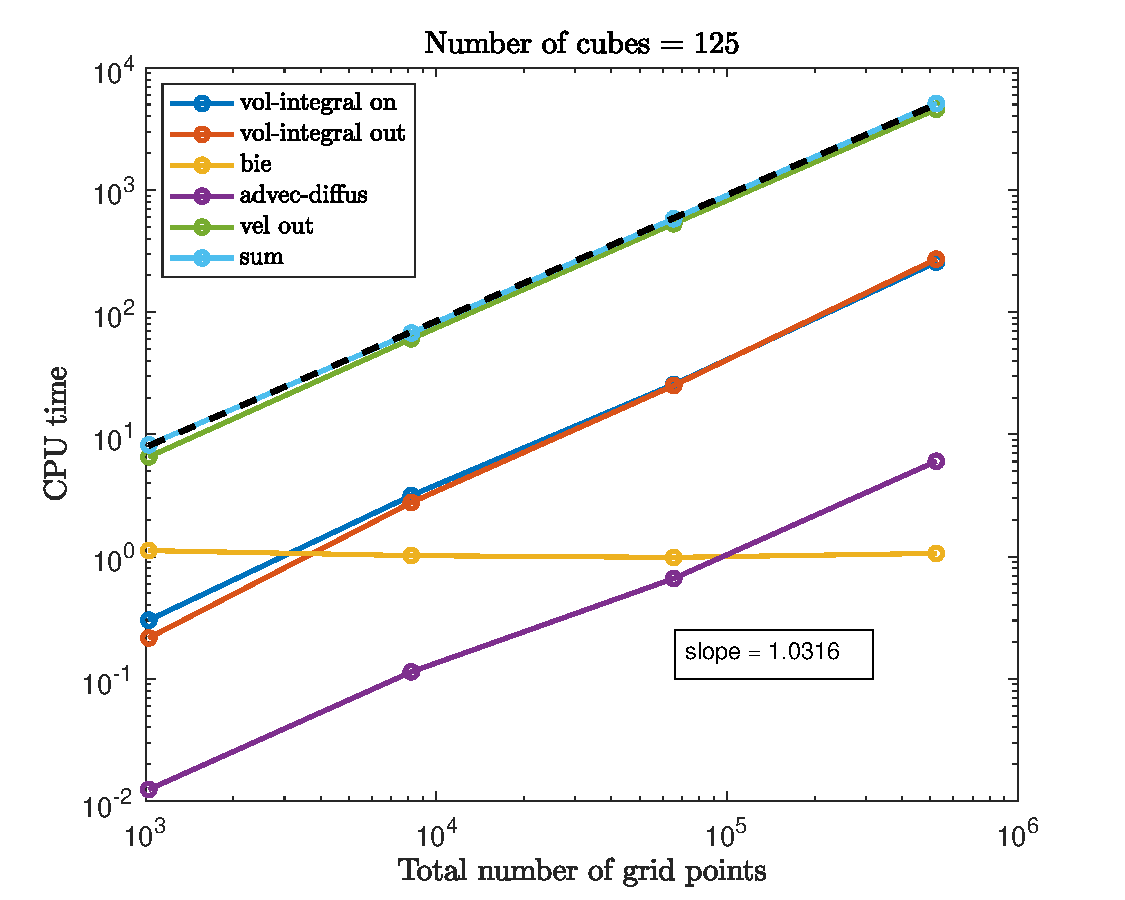
\includegraphics[scale=0.45]{./figures/fig_time_varNx5}
		% 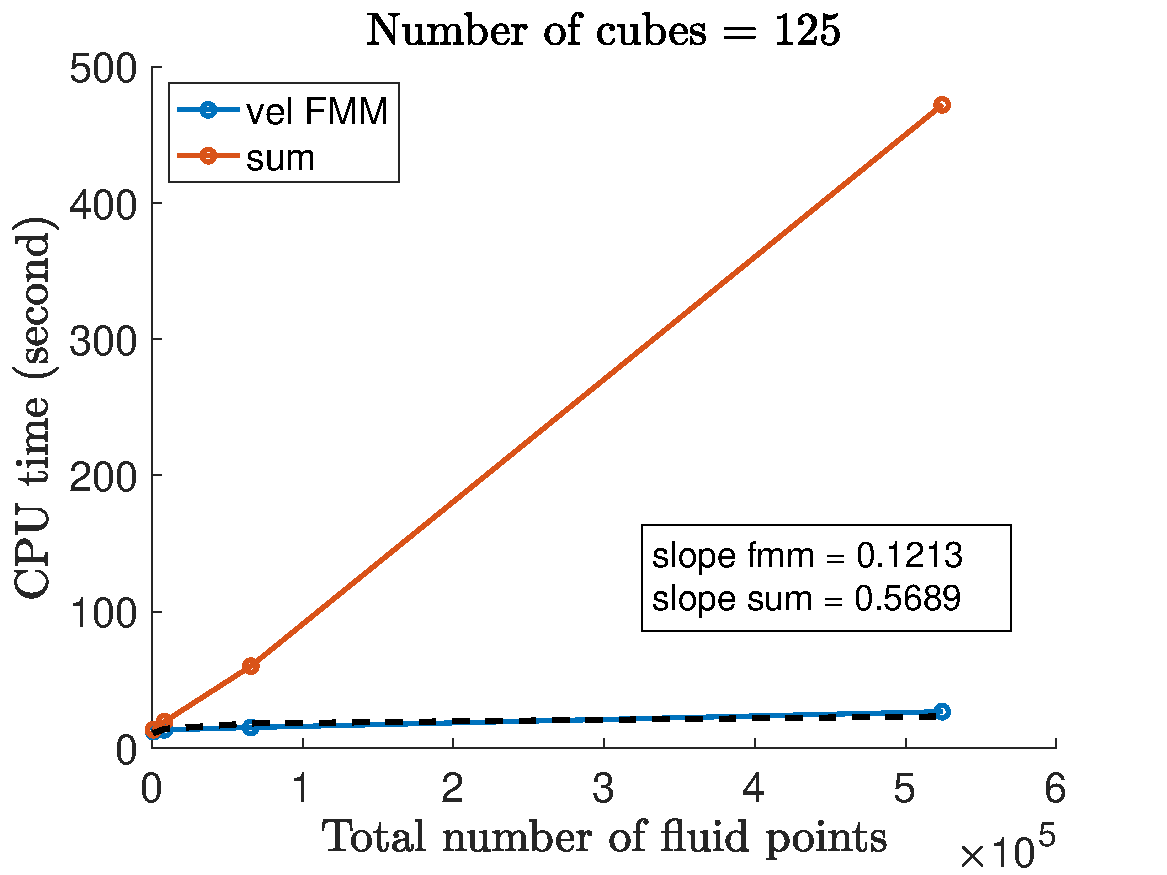
\includegraphics[scale=0.45]{./figures/fig_time_fmm_sum}
	\caption{CPU time in second with an aggregate of 125 cubes for ten time-steps.}
	\label{fig_time_fmm_sum}
\end{center}
\end{figure}
The main takeaway in this plot is that the velocity computation for all fluid points is dominant. 
We thus decided to use the FMM for this surface integral by approximating as follows:
Here, the points $\vec{x}$ are the sources, and $\vec{y}$ are the targets. 
For the velocity inside and on the aggregate boundary, we use the rigid boundary velocity $u(\vec{x}) = \vec{U}_a + \vec{\Omega} \times \left(\vec{x} - \vec{x}_{cm} \right)$. This implies that we only use targets located outside the aggregate, and we do not expect any singularity in this computation ($\vec{x} \neq \vec{y}$). However, we may have close evaluation problems. We will discuss the size of errors in the next section. 
\par
We handle the integration of the Stokeslet in a manner similar to what was done for the volume integral. 
Using the Laplace kernel, we can re-write the surface integral (\ref{eq_uH}) as
\begin{equation}
	u_H(\vec{y}) =
	\int_S 
	\vec{f}(\vec{x}) \cdot
  	\left(
  	\frac{\bar{\bar{I \ }}}{\|\vec{x} - \vec{y}\|}
  	- \left( \vec{x} - \vec{y} \right)
  	 \nabla_{\vec{y}}
  	\frac{1}{\|\vec{x} - \vec{y}\|}
  	\right)
	  \ \text{d} S(\vec{x}).
 \label{eq_surf_laplace}
\end{equation}
We first discretize the entire aggregate surface into $N_f$ square faces located at $[cx_j^n-1, cx^n_j+1]$, where $(cx^n_1, cx^n_2)$ is the center of $n-$th square face. The discretized version of the velocity equation (\ref{eq_surf_laplace}) is denoted by $H(\vec{y})$,
\begin{align}
	H(\vec{y}^m) & = u_H(\vec{y}) - E_f
	 = \sum_{n = 1}^{N_f} H^n(\vec{y}^m) 
	\nonumber \\
	& = \sum_{n = 1}^{N_f} 
	\vec{f}(\vec{x}^n) \cdot
	\int_{cx^n_2-1}^{cx^n_2+1} \int_{cx_1^n-1}^{cx_1^n+1}
  	\left(
  	\frac{\bar{\bar{I \ }}}{\|\vec{x}^n - \vec{y}^m\|}
  	- \left( \vec{x}^n - \vec{y}^m \right)
  	 \nabla_{\vec{y}^m}
  	\frac{1}{\|\vec{x}^n - \vec{y}^m\|}
  	\right)
	  \text{d} x_1  \text{d} x_2
	  ,
 \label{eq_surf_fmm_N_f}
\end{align}
where the error coming from this approximation is denoted as $E_f$. A more detailed analysis regarding $E_f$ can be found in section \ref{sec:bie_validataion}.
 Note that the stress $\vec{f}(\vec{x}^n)$ is assumed to be constant over each square face.  One can find that we have a significant error in the cube's corners. We want to ensure that we do not introduce larger errors as we make further approximations. 

\par
Next, we need to approximate the surface integral in equation (\ref{eq_surf_fmm_N_f}) using a Riemann sum,
\begin{align}
	\tilde{H}(\vec{y}^m) 
	& = H^n(\vec{y}^m) - E_{G} 
	\nonumber \\ 
	& =
	\sum_{n = 1}^{N_f} 
	\vec{f}(\vec{x}^n) \cdot
	\sum_{s=1}^{Ns^2} d^2 
  	\left(
  	\frac{\bar{\bar{I \ }}}{\|\vec{x}_s^n - \vec{y}_s^m\|}
  	- \left( \vec{x}_s^n - \vec{y}^m \right)
  	 \nabla_{\vec{x}_s^n}
  	\frac{1}{\|\vec{x}_s^n - \vec{y}^m\|}
  	\right)
	  - E_{G},
 \label{eq_surf_fmm_N_f_n}
\end{align}
where $E_G$ is the error coming from the quadrature method. 
We use $N_s^2$ sub-squares with sizes of $d = 2/N_s$, and take the center of each sub-squares as the integration point. 
We take the same number of points, $N_s$, evenly distributed in one direction. 
In the following schematics, Figure \ref{fig_face_grid}, the red cross represents the center of the $n-$th square face, $(cx^n_1, cx^n_2)$.
\begin{figure}[h]
	\begin{center}
		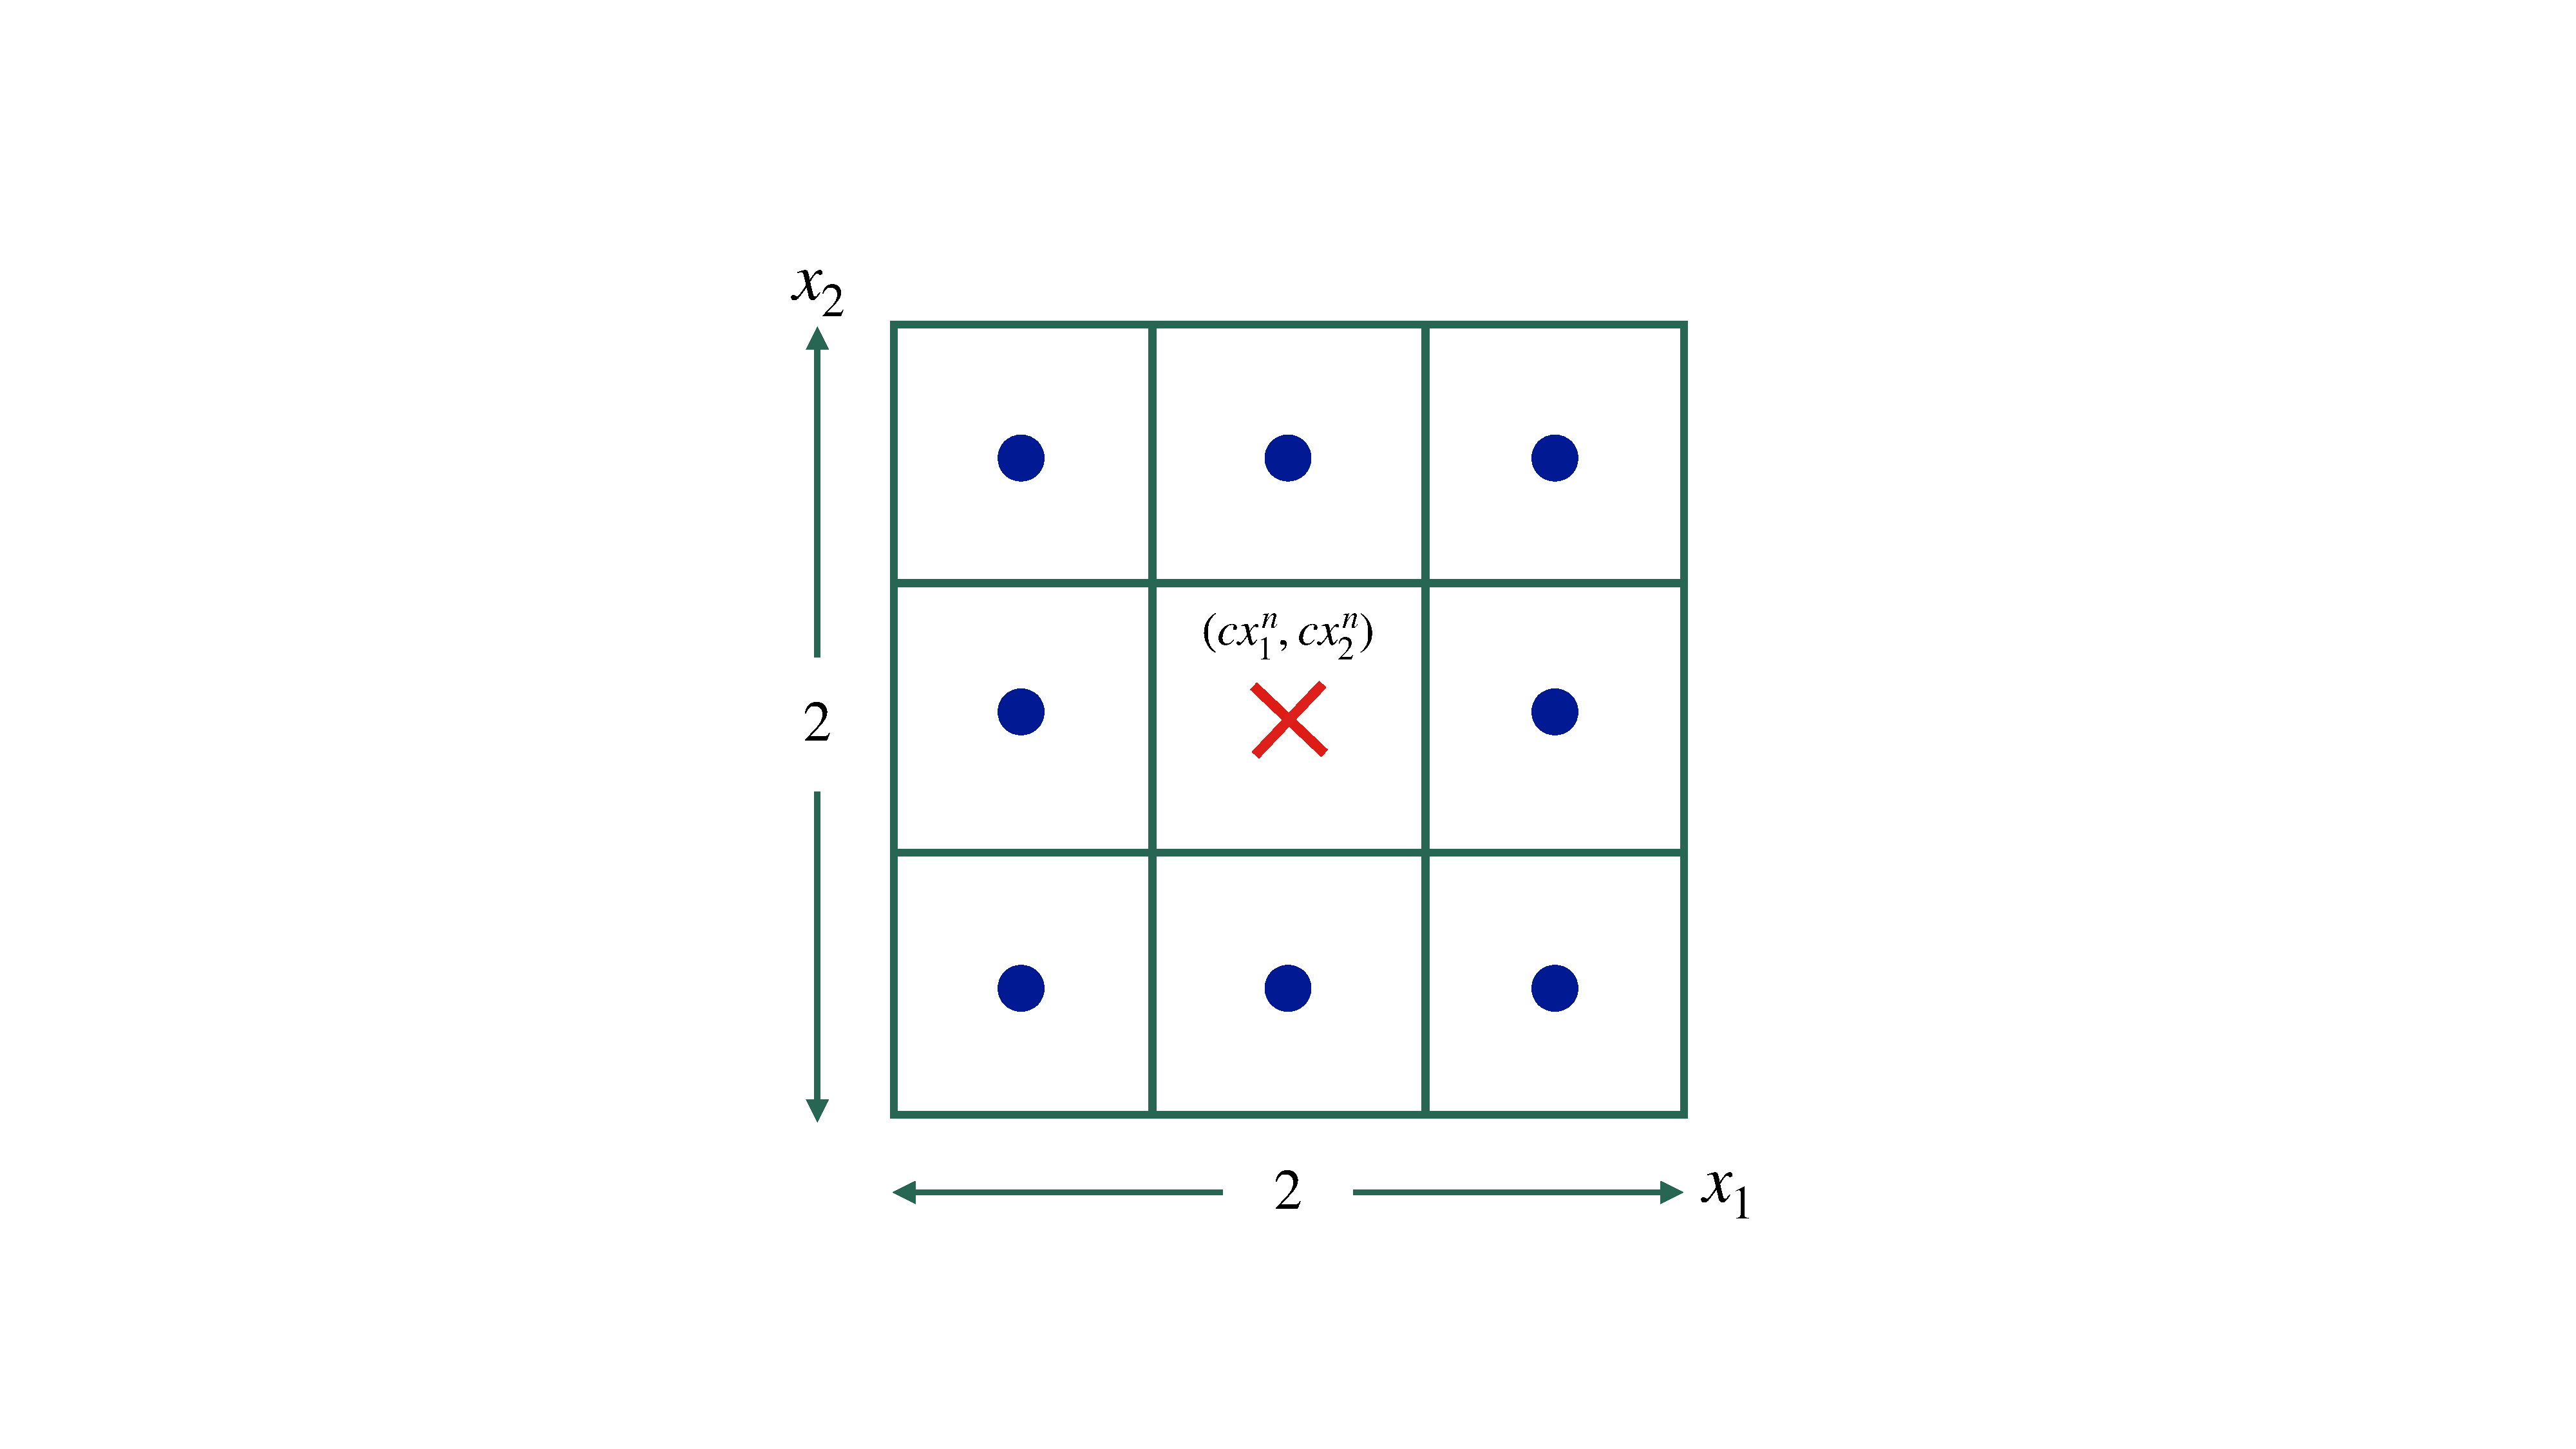
\includegraphics[scale=0.17]{./figures/fig_face_grid}
	\caption{Schematic of points we use to approximate the integral of the single-layer potential kernel over one square face.}
	\label{fig_face_grid}
\end{center}
\end{figure}
The blue dots and the red cross are the integration points.
We do not include any boundary values on one square face for simplicity.
\par
As mentioned, we hope to have a reasonable size of the integration error, i.e., $E_G \ll E_f$.
To measure $E_f$, we consider the settling of one cube shape aggregate.
We then observe the relative error of the vertical velocity on one square face, considering the translational velocity, $\vec{U}_a$, as the exact solution.
\begin{figure}[h]
	\begin{center}
		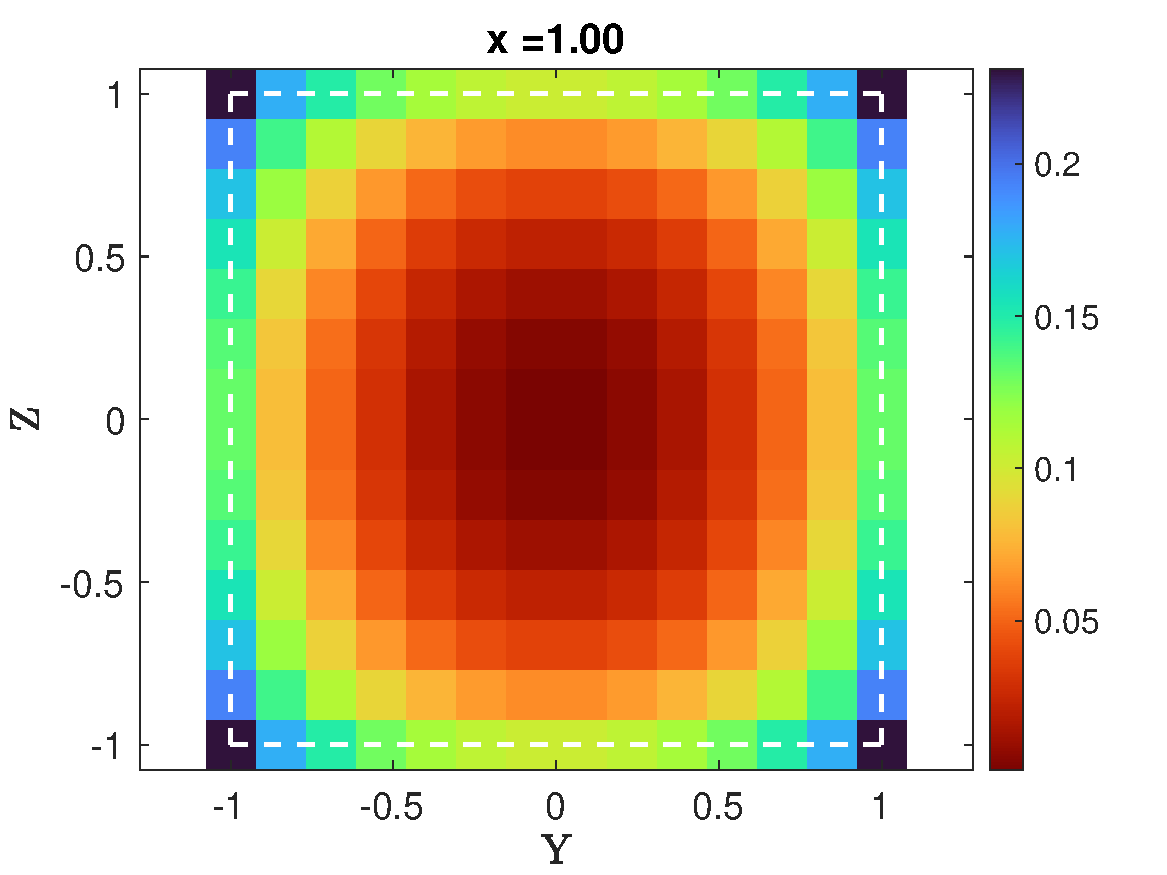
\includegraphics[scale=0.3]{./figures/fig_corner_err}
	\caption{Sample case of the relative velocity error on one face, $E_f$.}
	\label{fig_corner_err}
\end{center}
\end{figure}
In Figure \ref{fig_corner_err}, we see the square face at $x = 1$, where the white dashed line shows the location of the square face, and the color indicates the relative error. It implies that the maximum of 23.12$\%$ error occurs at the cube's corner, as we expected. We thus would like to regulate the quadrature error, $E_G$, by adjusting the total number of integration points, $Ns^2$.
\par
Two parameters affect the efficiency and accuracy of the FMM computations: 1) the number of quadrature points and 2) the tolerance $\varepsilon$ in the FMM3D library, which determines the number of terms in the series expansion.
In Figure \ref{fig_Ef_EG_compare}, we vary the number of integration points to choose an optimal value. 
\begin{figure}[ht]
	\begin{center}
		% 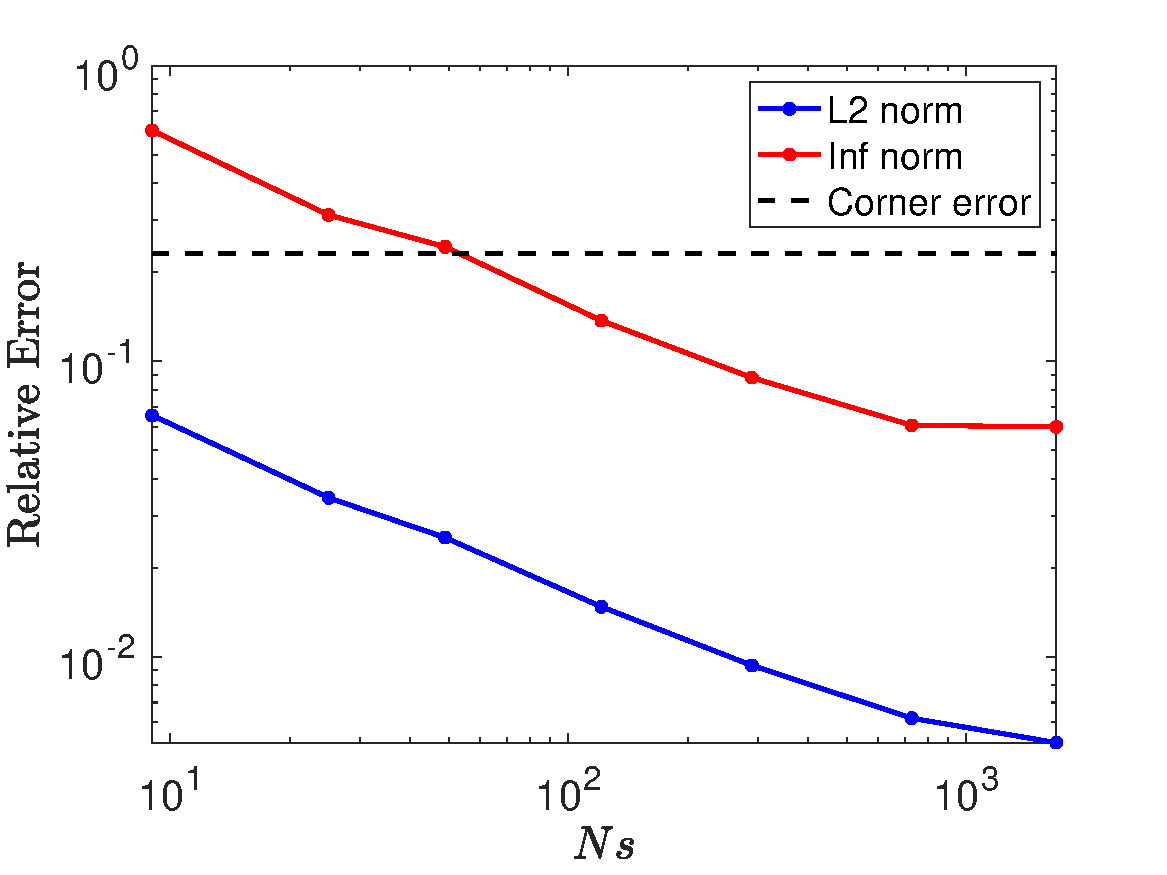
\includegraphics[scale=0.33]{./figures/fig_Ef_EG_compare}
		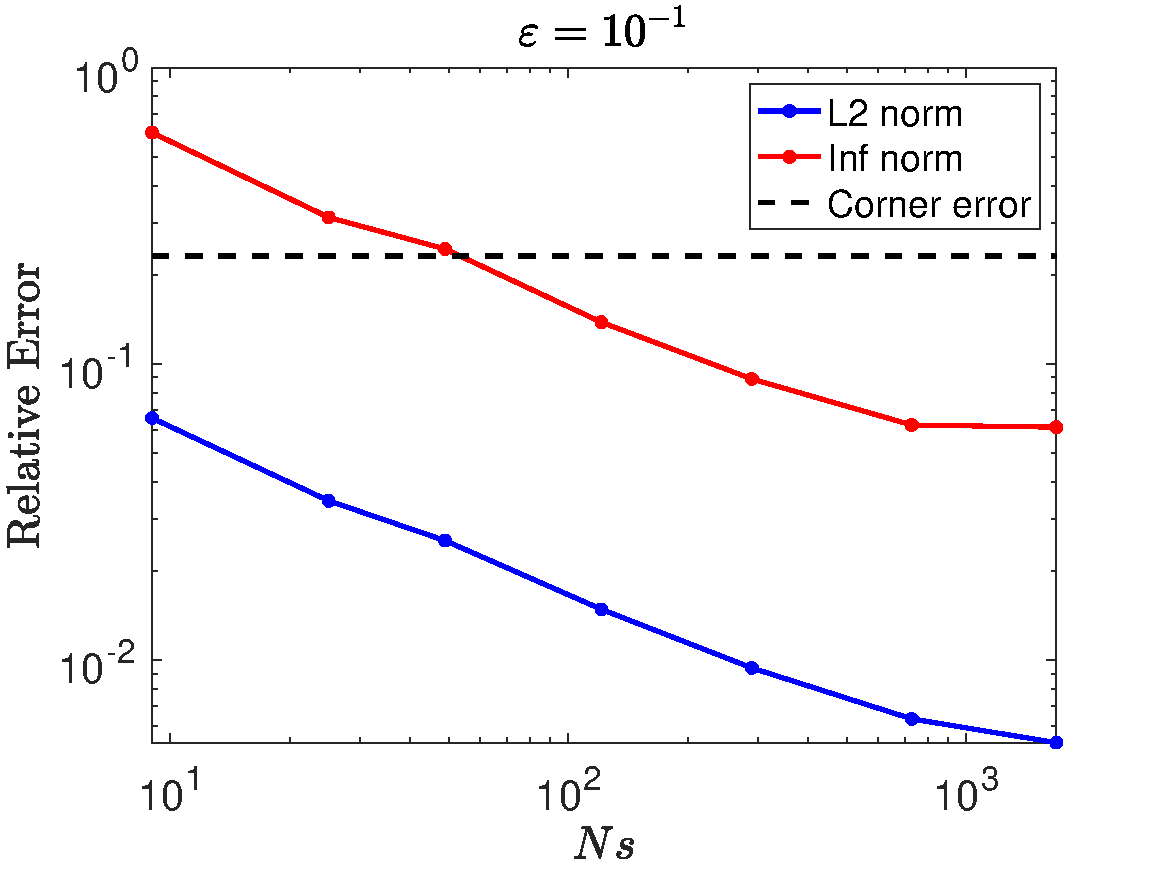
\includegraphics[scale=0.45]{./figures/fig_Ef_Eg_ep-1}
	\caption{Relative error between $U^*$ and $U^{*+}$, varying the number of integration points: $Ns = [3, 5, 7, 11, 17, 27,41]^2$ and $\varepsilon = 10^{-1}$.}
	\label{fig_Ef_EG_compare}
\end{center}
\end{figure}
We test a single-time simulation in the domain,  $[-5, 5] \times [-5, 5] \times [-10, 10]$,  with one cube aggregate model. To confirm the responses of $\varepsilon$ values, we simulate the same one with two tolerance values, $\varepsilon = 10^{-1}, \ 10^{-6}$.
From this analysis, we are convinced that $Ns = 9^2$ quadrature points are enough to satisfy the error size we can tolerate. It produces quite similar results for the $\varepsilon = 10^{-6}$ case. We did not notice any difference in accuracy. We may observe this because the corner error, $E_f$, dominates our approximation and is already larger than $10 \%$. 

After implementing the FMM3D library into our program, we timed one more time to compare the fluid velocity computation shown as the green (or dashed line) in Figure \ref{fig_time_fmm_sum}. The efficiency of the computation increases about ten times when the number of fluid grid points is about 500,000, which is in the range of what we will use to compute the fully stratified simulations.
\begin{figure}[ht]
	\begin{center}
		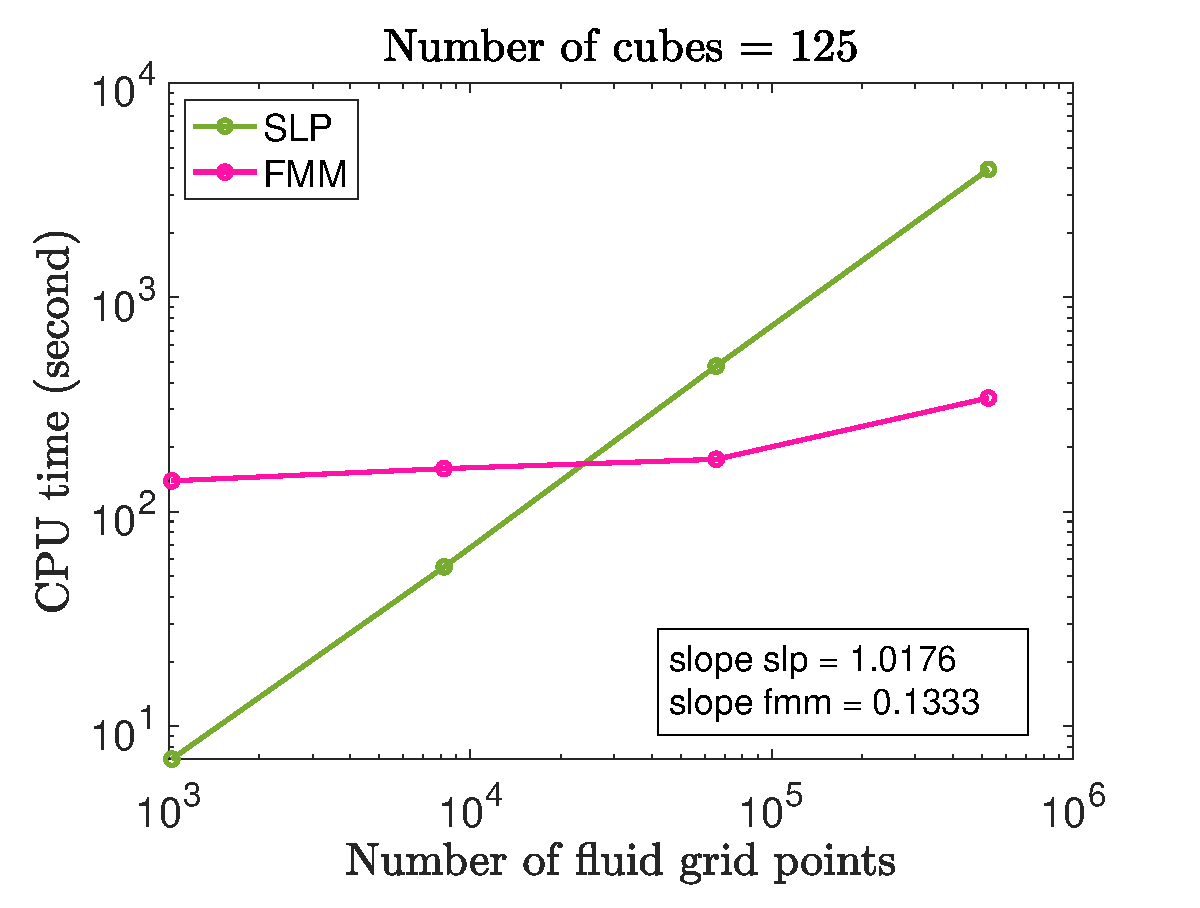
\includegraphics[scale=0.45]{./figures/fig_time_both_mm5_Nt10}
	\caption{CPU time with an aggregate made with 125 cubes for ten time steps. The green line is the velocity computation with the original single-layer potential code, and the pink line represents the approximation using the FMM3D library.}
	\label{fig_vel_mm5_t1}
\end{center}
\end{figure}


%validation---------------------------------------------------
\section{Validation}
In order to determine our simulation settings, we examine the simplified results by varying 1) time step $\Delta t$, 2) space step $\Delta x$, and 3) domain sizes. Note that we use uniform spacing for all directions, i.e., $\Delta x = \Delta y = \Delta z$. To differ the fluid domain size, we consider the center of mass,  $\vec{x}_{cm}$, and the maximum radius of the aggregate, $R_m$.
From $\vec{x}_{cm}$, we scale the domain $V$ with a constant $s$,
\[
	V = 
	\begin{bmatrix}
	 \ \vec{x}_{cm} - \begin{pmatrix}
		1 \\ 1 \\ 2
		\end{pmatrix} s R_m , 
		\ \vec{x}_{cm} + \begin{pmatrix}
			1 \\ 1 \\ 2
			\end{pmatrix} s R_m.
	\end{bmatrix}
\]
\begin{figure}[ht]
	\begin{center}
		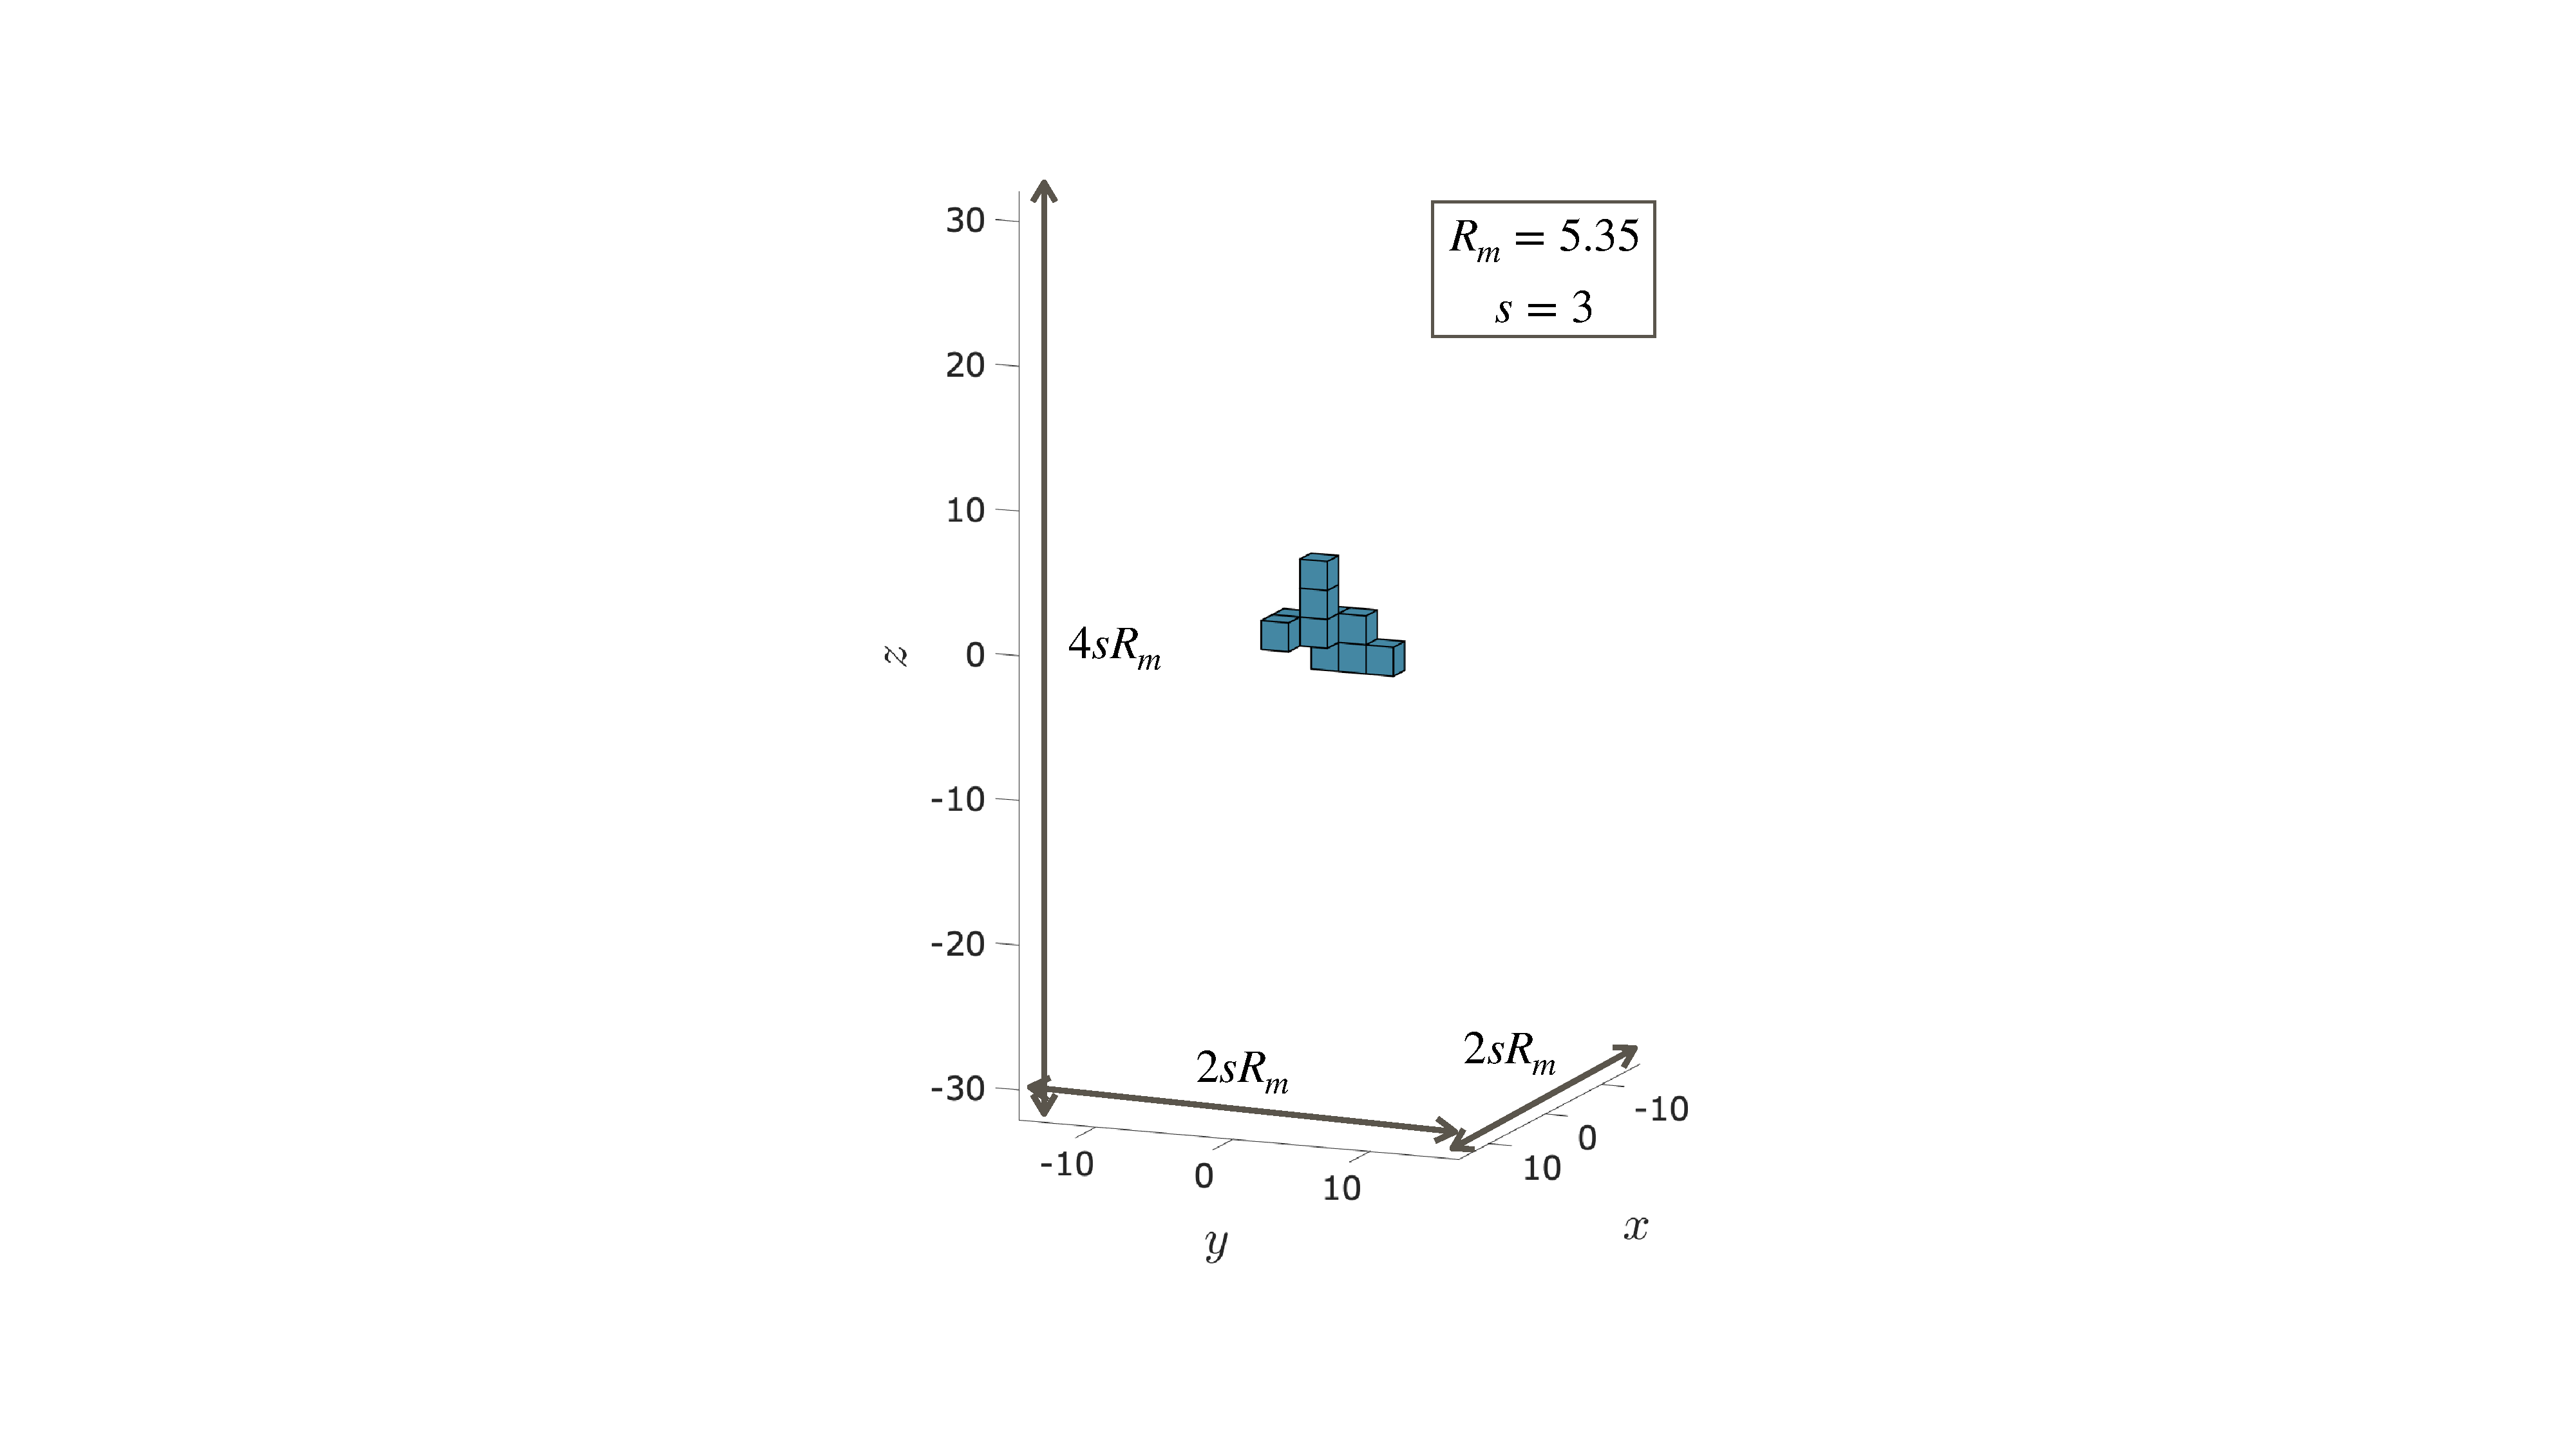
\includegraphics[scale=0.45]{./figures/fig_sample_agg10.pdf}
		\caption{Sample aggregate with ten cubes. This model is used to obtain simulations presented in Figure \ref{fig_NC10_snaps_all}.}
		\label{fig_sample_agg10}
	\end{center}
\end{figure}
We use ten cubes to form an aggregate model for the validation, as shown in Figure \ref{fig_sample_agg10}.
Since we are interested in the aggregate's behavior, we measure its translational velocity $\vec{U}_a$, location of $\vec{x}_{cm}$, and drag. The sole fluid quantity we want to observe is the perturbation $C(\vec{x},t)$. At a location that is far away from the aggregate, we expect to see very small, almost zero, perturbation.
We thus focus on the perturbation value near the aggregate.
\par
\begin{figure}[ht]
	\begin{center}
		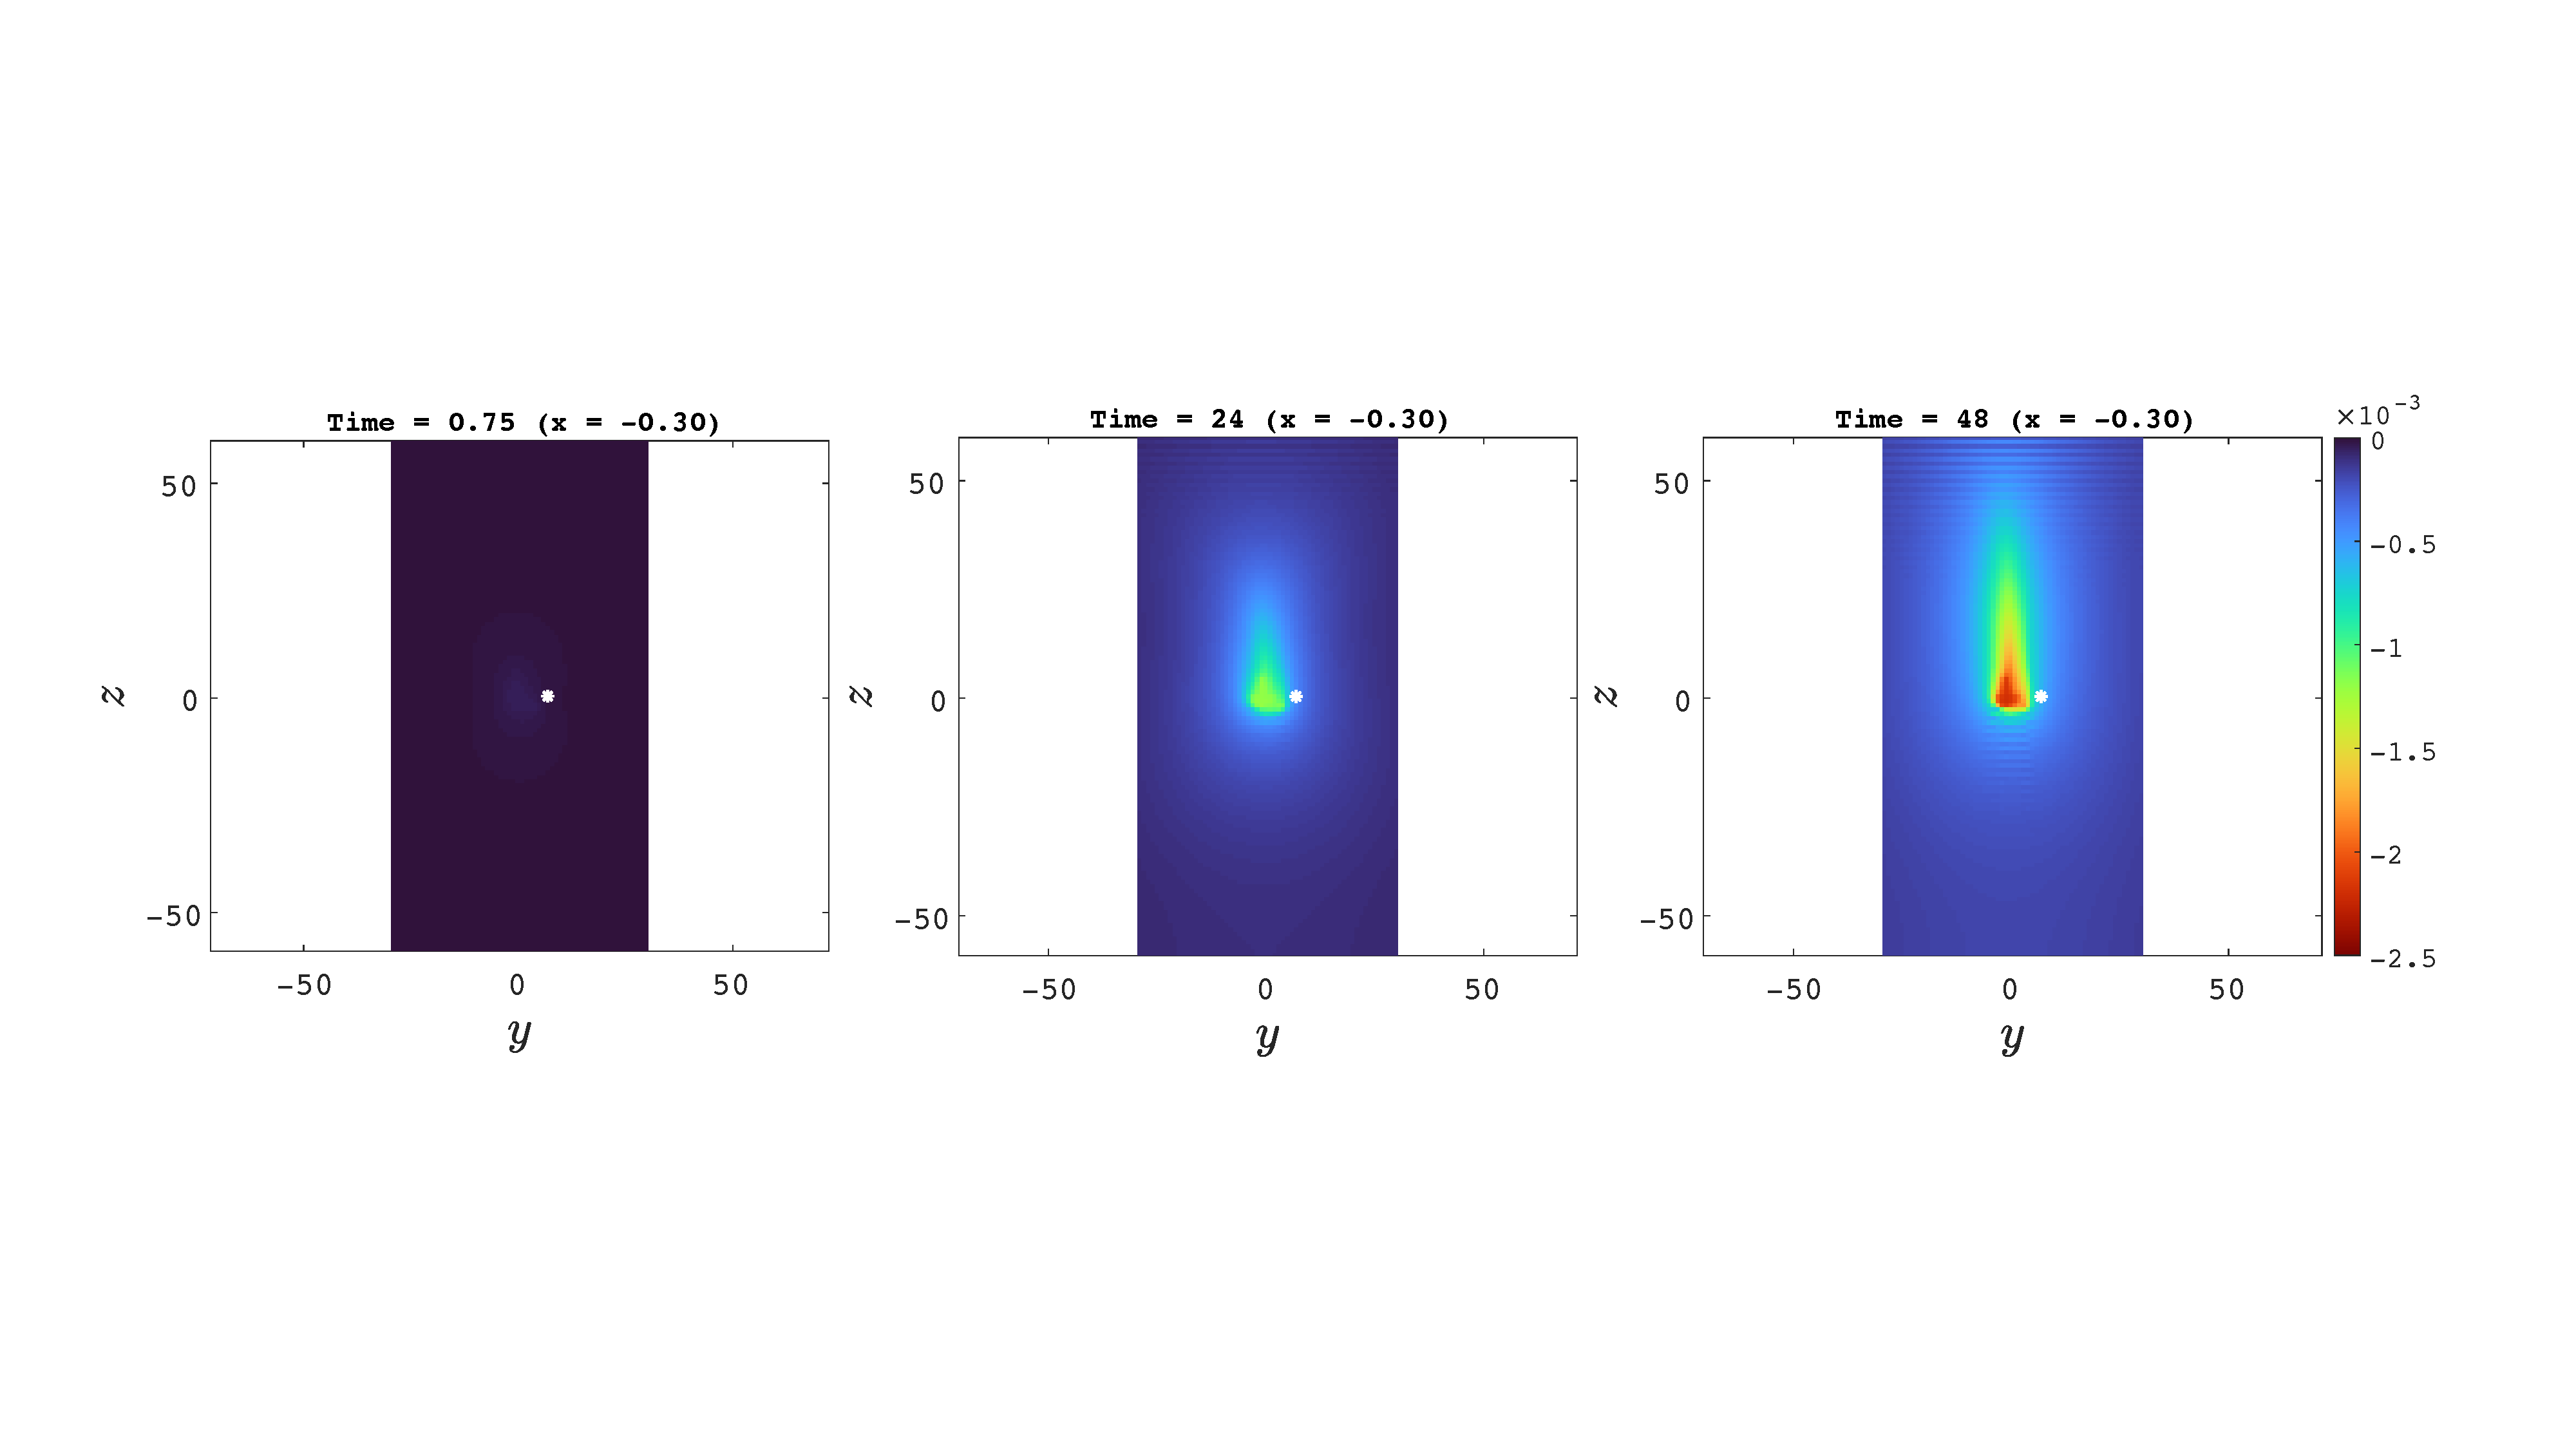
\includegraphics[scale=0.235]{./figures/fig_NC10_snaps_all.pdf}
		\caption{Snapshots of the perturbation obtained with $\Delta t = 0.75, \ \Delta x = 1,$ and $s = 5$. We look at $y-z$ plane at $x = -0.3$, which is near the center of mass of the aggregate. The small white dot is located outside of, but very close to, the aggregate.}
		\label{fig_NC10_snaps_all}
	\end{center}
\end{figure}
As a sample result, Figure \ref{fig_NC10_snaps_all} shows three snapshots of the perturbation $C$, obtained with $\Delta t = 0.75, \ \Delta x = 1$, and $s = 5$, at $x = -0.3$. Note that the white star point is $(-0.3, \    6.9, \      0.4)$. Since we use the moving frame of reference to compute the perturbation, the aggregate stays in the middle of the fluid domain in Figure \ref{fig_NC10_snaps_all}.
We notice slight instabilities on the top of the fluid domain, where the zero-flux boundary condition is applied, as the perturbation increases. Considering a large enough fluid domain compared to the aggregate size, we would like to observe the convergence of the quantities of interest near the aggregate. 
\subsection{Various time sizes}
The main takeaway of these plots is that there are no significant differences in values we observe. Although we notice some variations of the perturbation at a later time, it essentially goes to zero as the aggregate and surrounding fluid densities become neutral. 
\begin{figure}[ht]
	\begin{center}
		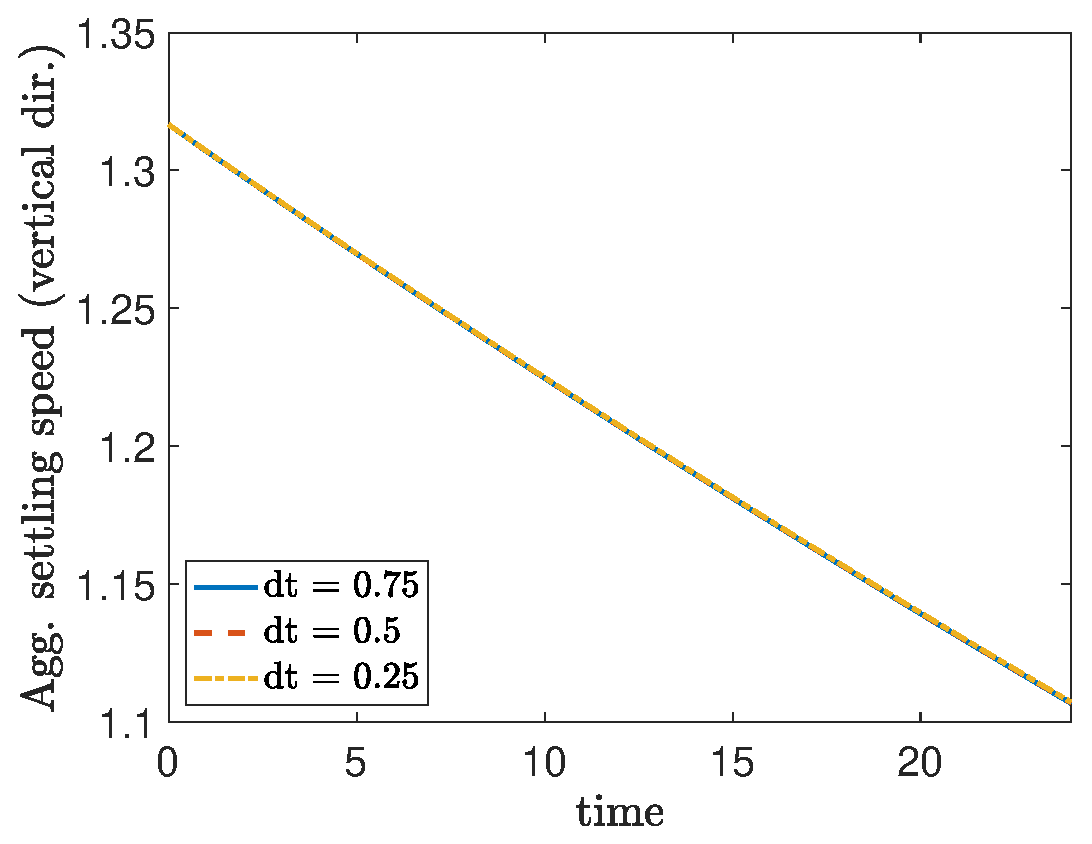
\includegraphics[scale=0.35]{./figures/fig_NC10_dt_Ua3_all}
		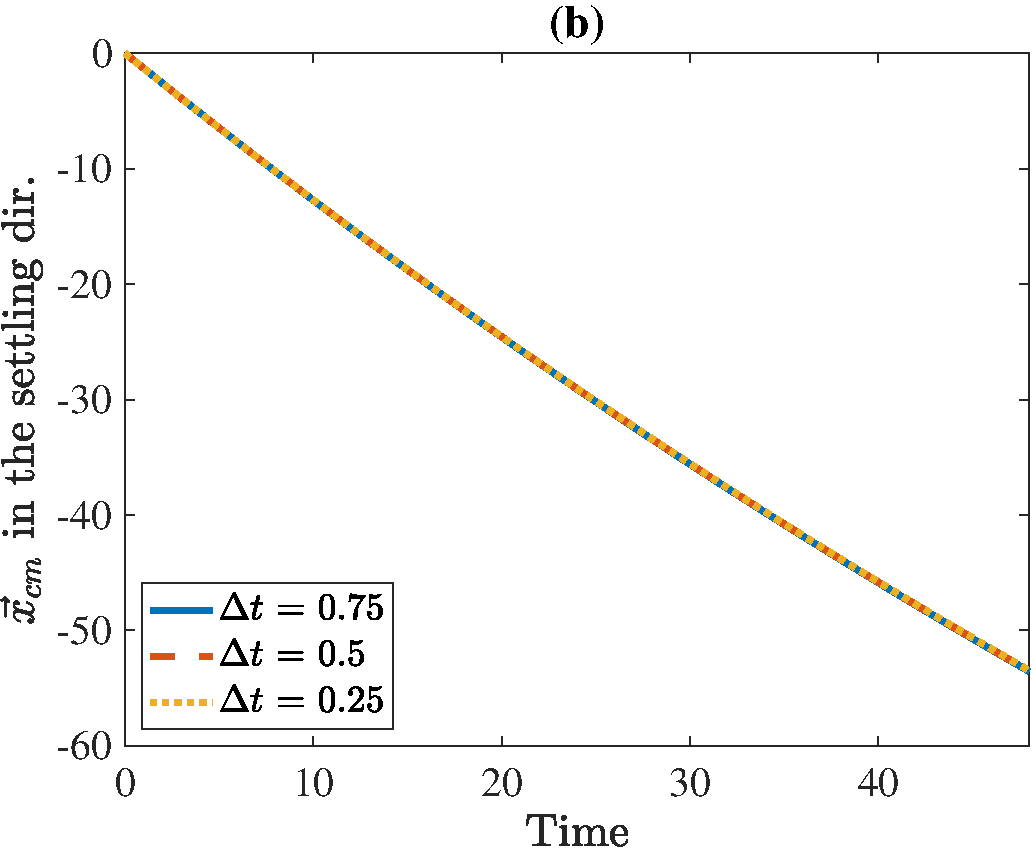
\includegraphics[scale=0.35]{./figures/fig_NC10_dt_cm3_all}
		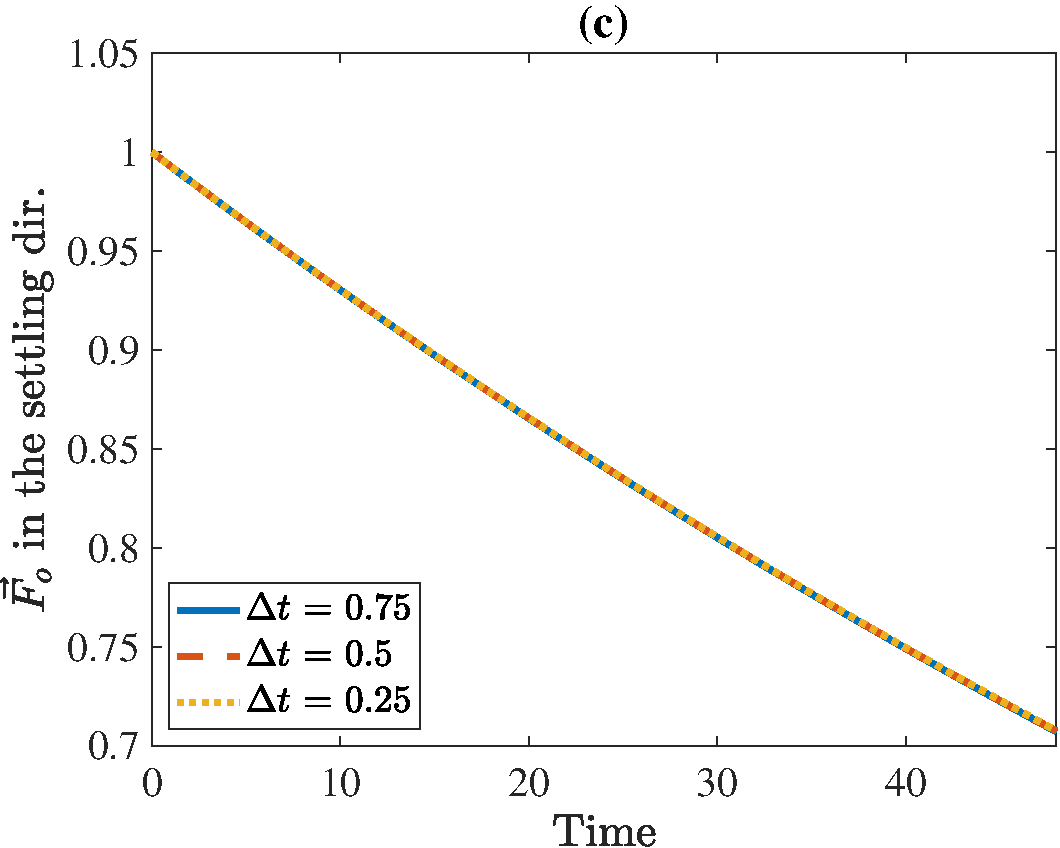
\includegraphics[scale=0.35]{./figures/fig_NC10_dt_Fo3_all}
		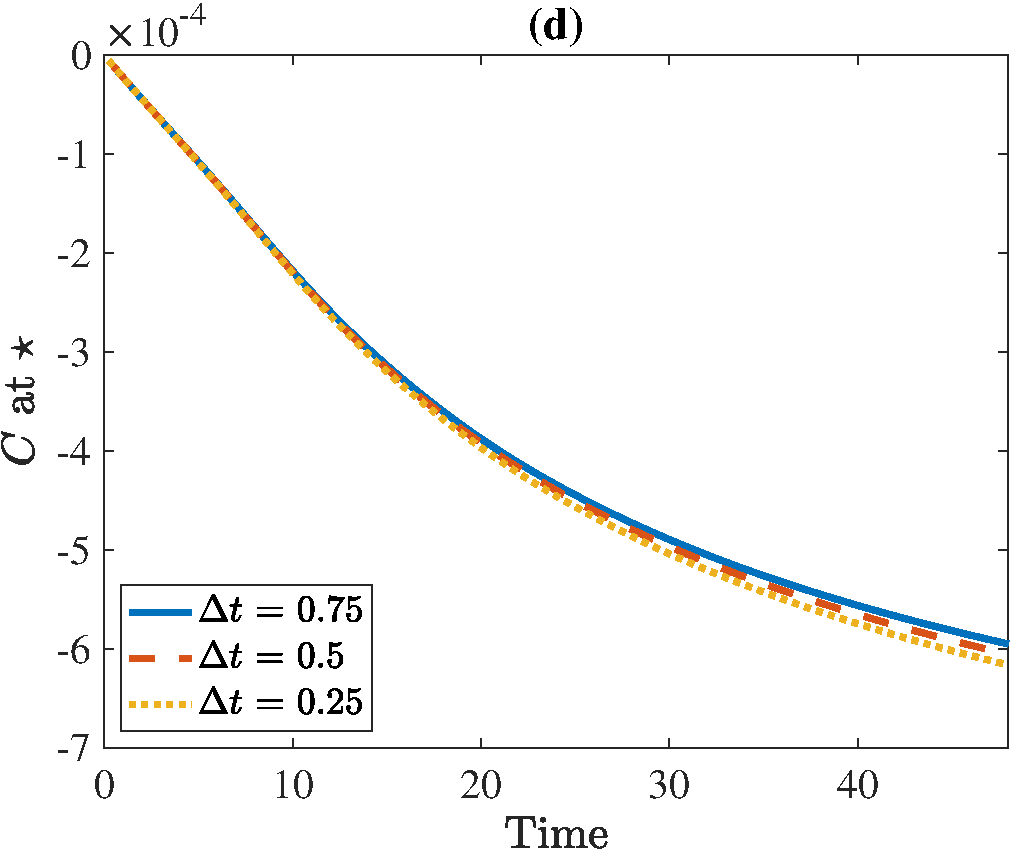
\includegraphics[scale=0.35]{./figures/fig_NC10_dt_C_star}
	\caption{Compare various $\Delta t = 0.75, \ 0.5, \ 0.25$ in the domain size factor $s = 5$ with $\Delta x = 1$.}
	\label{fig_NC10_compare_dt}
\end{center}
\end{figure}

\subsection{Various space sizes}
Once we are convinced that we can find useful information at locations with $\Delta x = 4$, it would accelerate our computation time. The fewer points we use, the more time we can save. We see the perturbation plots that are not convergent because we could not capture the perturbation at the same location. 
\begin{figure}[ht]
	\begin{center}
		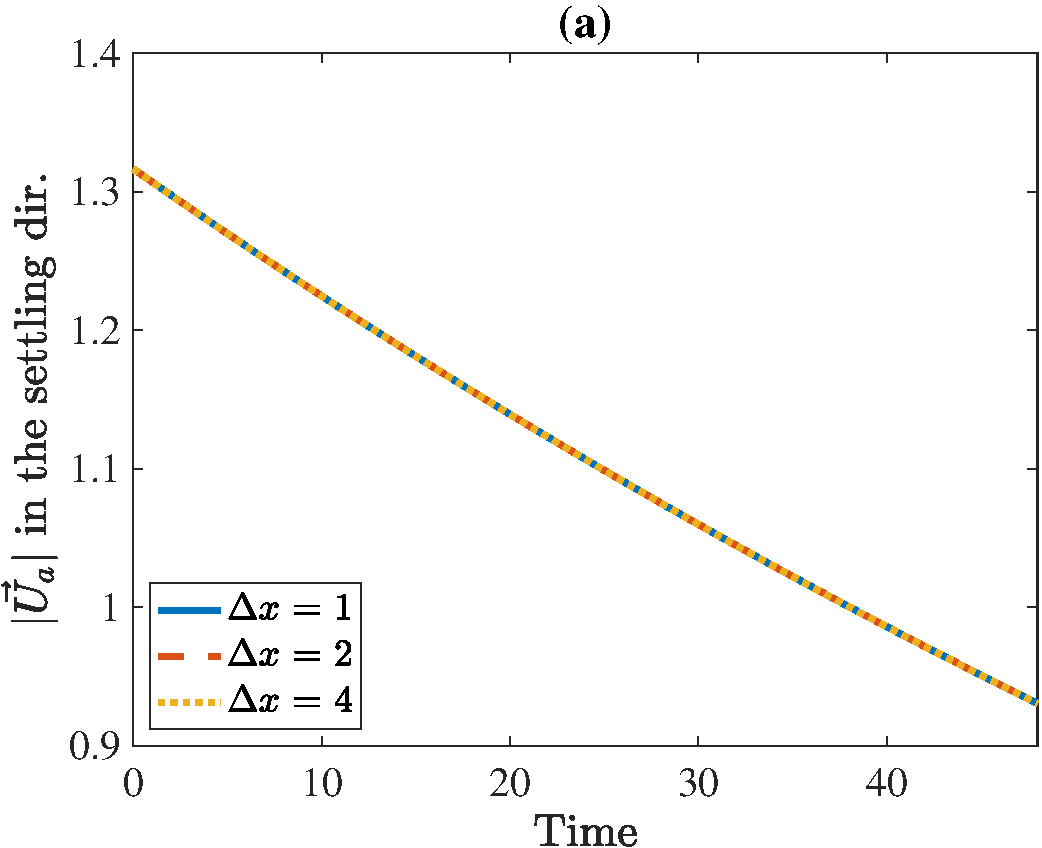
\includegraphics[scale=0.35]{./figures/fig_NC10_dx_Ua3_all}
		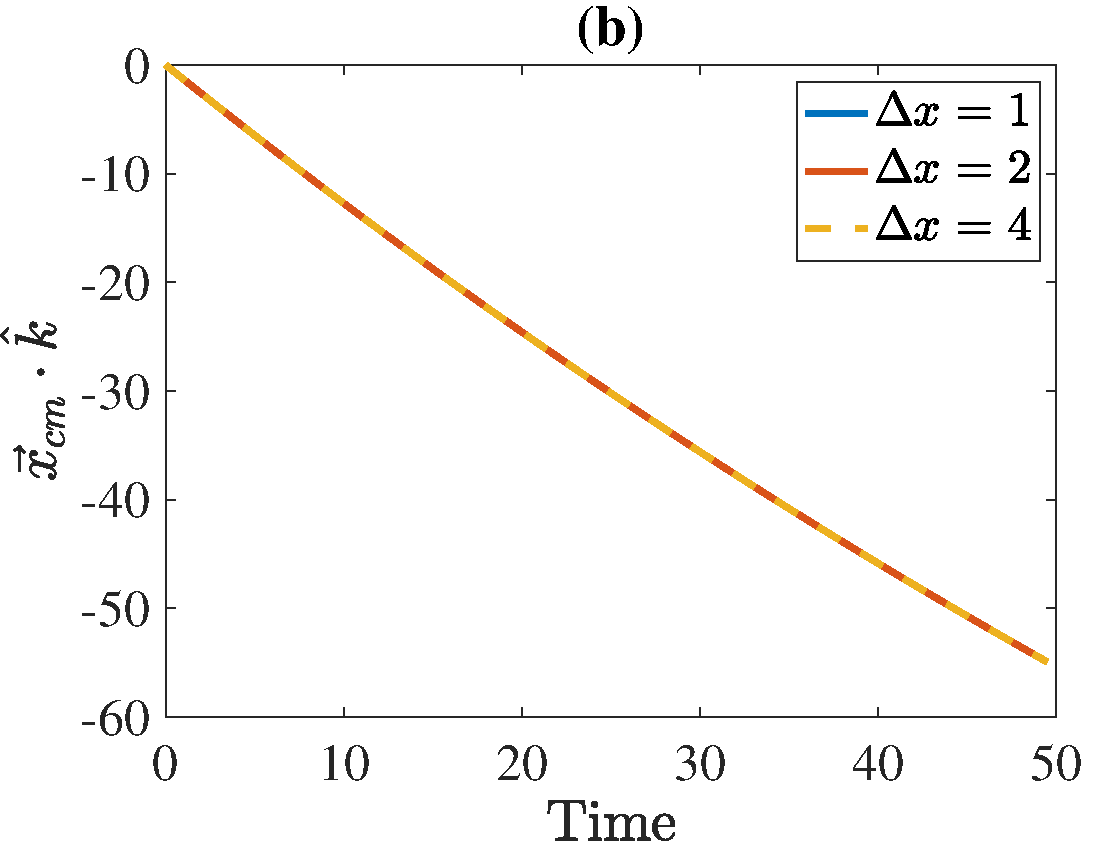
\includegraphics[scale=0.35]{./figures/fig_NC10_dx_cm3_all}
		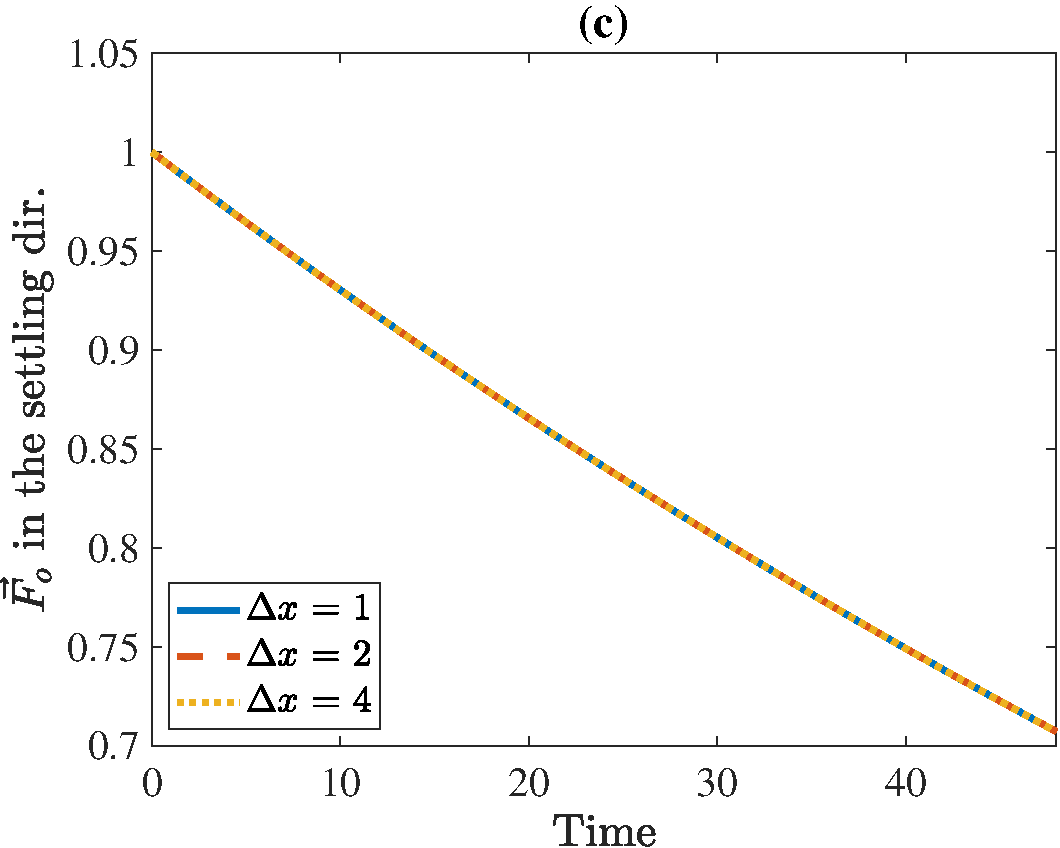
\includegraphics[scale=0.35]{./figures/fig_NC10_dx_Fo3_all}
		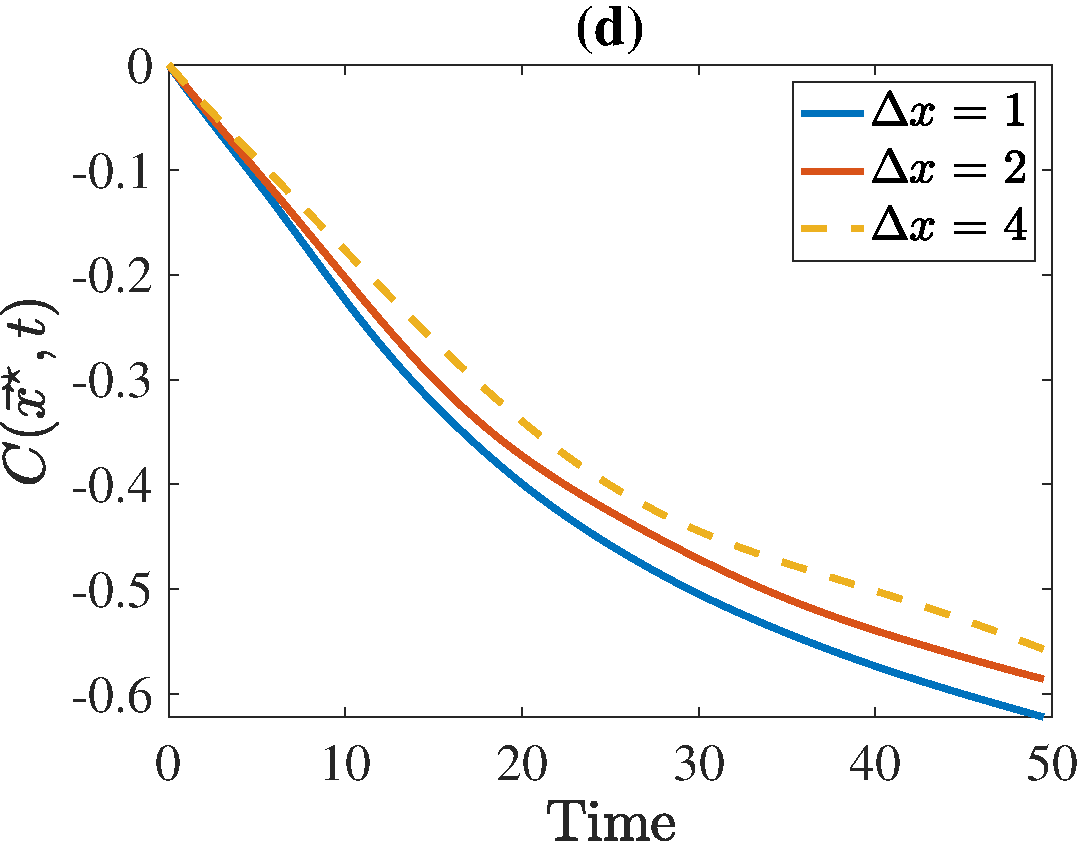
\includegraphics[scale=0.35]{./figures/fig_NC10_dx_C_star}
	\caption{Compare various $\Delta x = 1, \ 2, \ 4$ in the domain size factor $s = 5$ with $\Delta t = 0.75$.}
	\label{fig_NC10_compare_dx}
\end{center}
\end{figure}
\subsection{Various domain sizes}
We want to see whether the dynamics change drastically when we put our aggregate in a smaller box. We assumed to have $s = 5$ for all simulations. It is worthwhile to examine different $s$ scales in case we need more rapid computations. 
\begin{figure}[ht]
	\begin{center}
		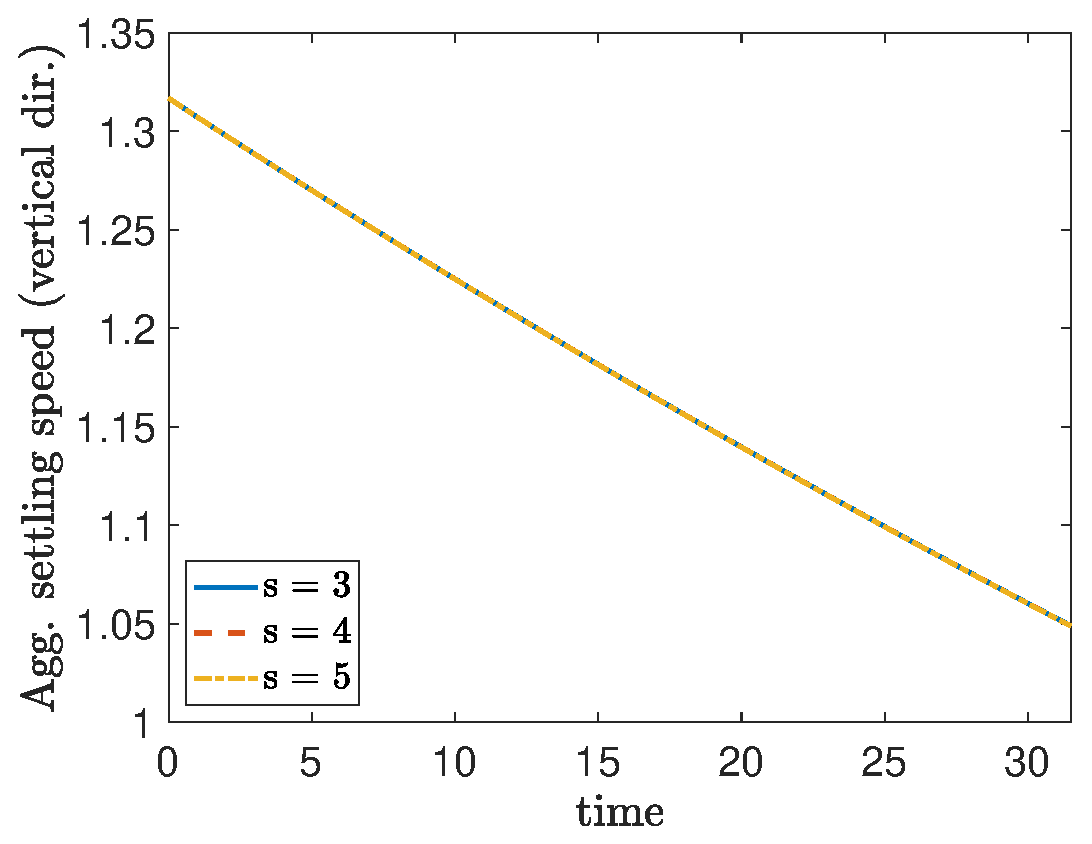
\includegraphics[scale=0.33]{./figures/fig_NC10_s_Ua3_all}
		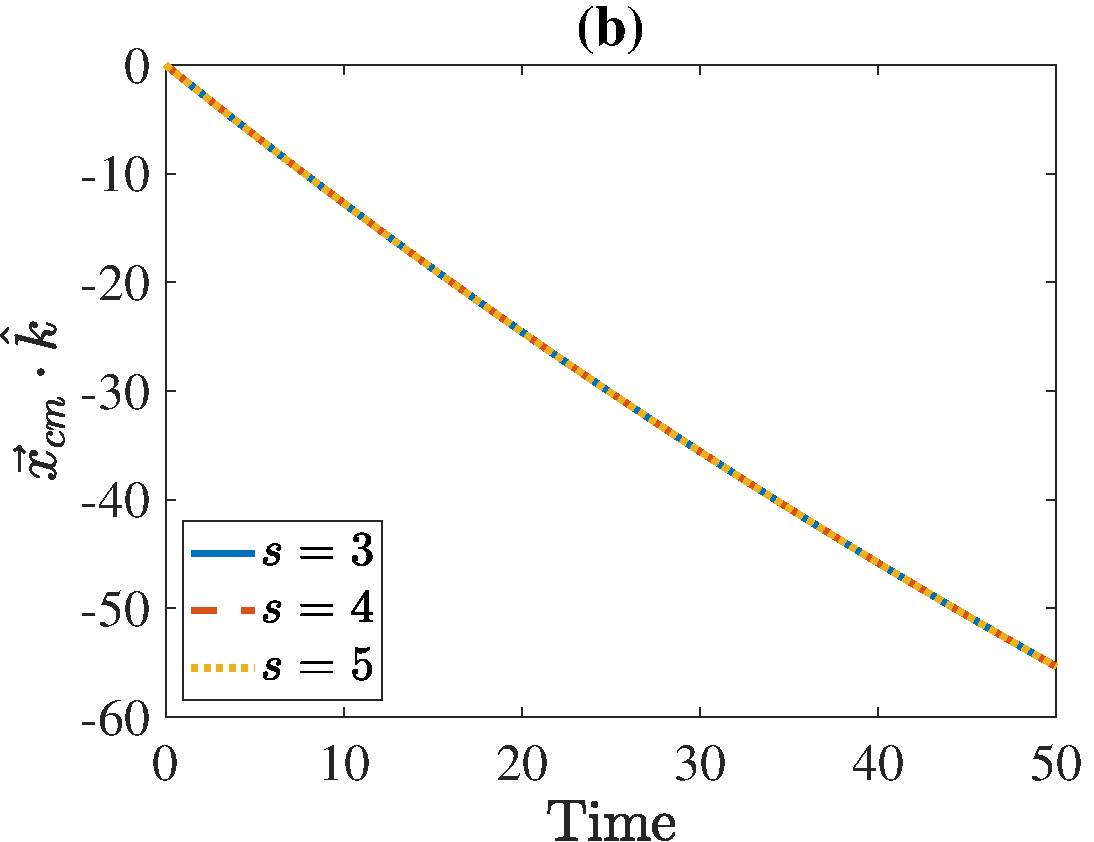
\includegraphics[scale=0.33]{./figures/fig_NC10_s_cm3_all}
		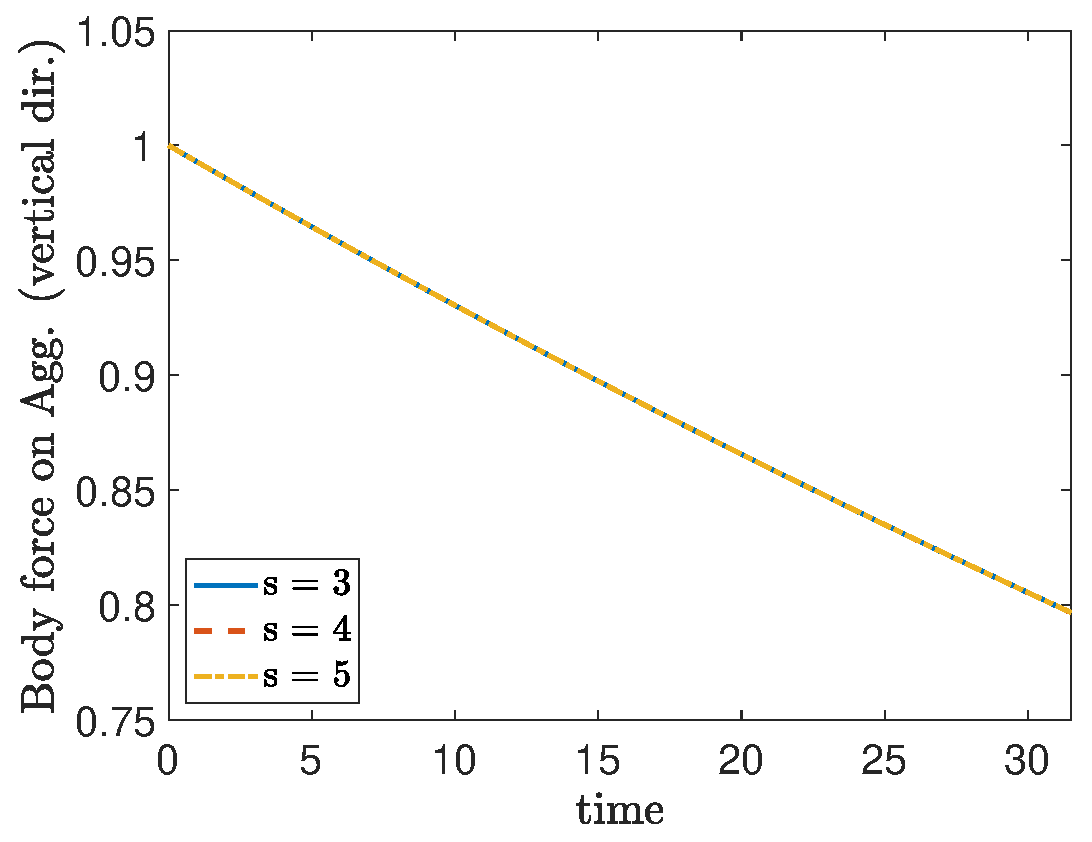
\includegraphics[scale=0.33]{./figures/fig_NC10_s_Fo3_all}
		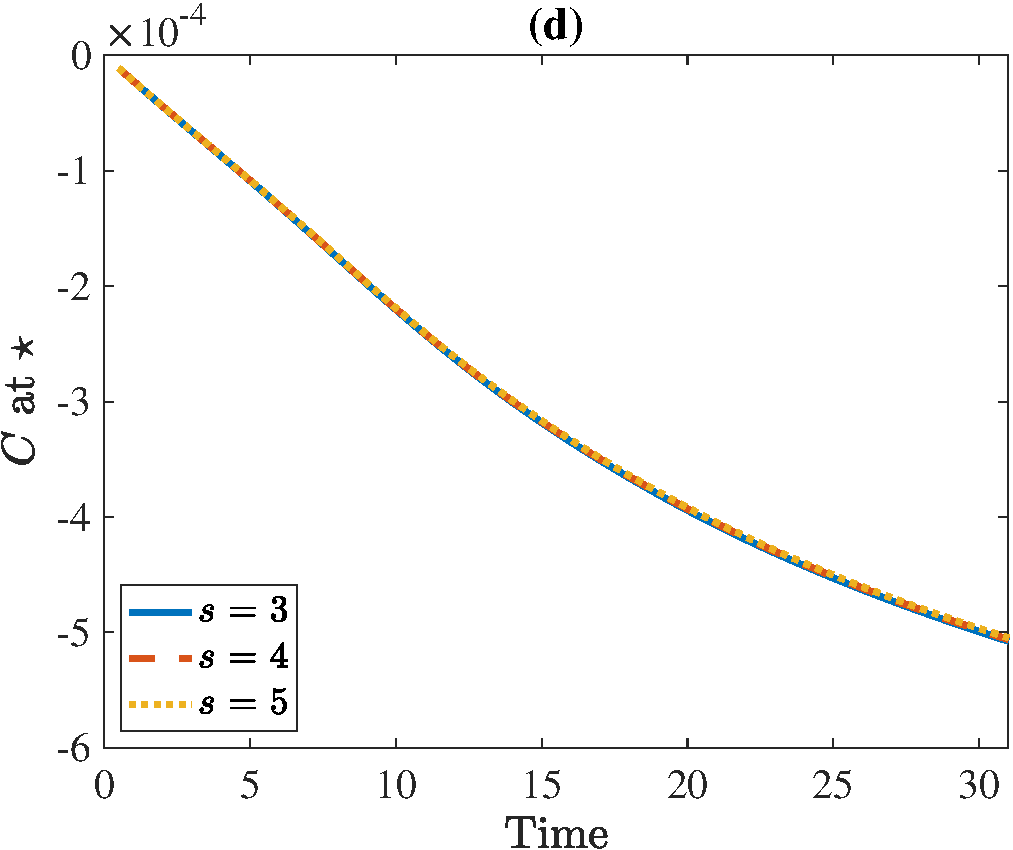
\includegraphics[scale=0.33]{./figures/fig_NC10_s_C_star}
	\caption{Compare various domain sizes $\Delta s = 3, \ 4, \ 5$ in the step sizes $\Delta t = 0.5$ with $\Delta x = 1$.}
	\label{fig_NC10_compare_s}
\end{center}
\end{figure}


Fifty cube samples.
\begin{figure}[ht]
	\begin{center}
		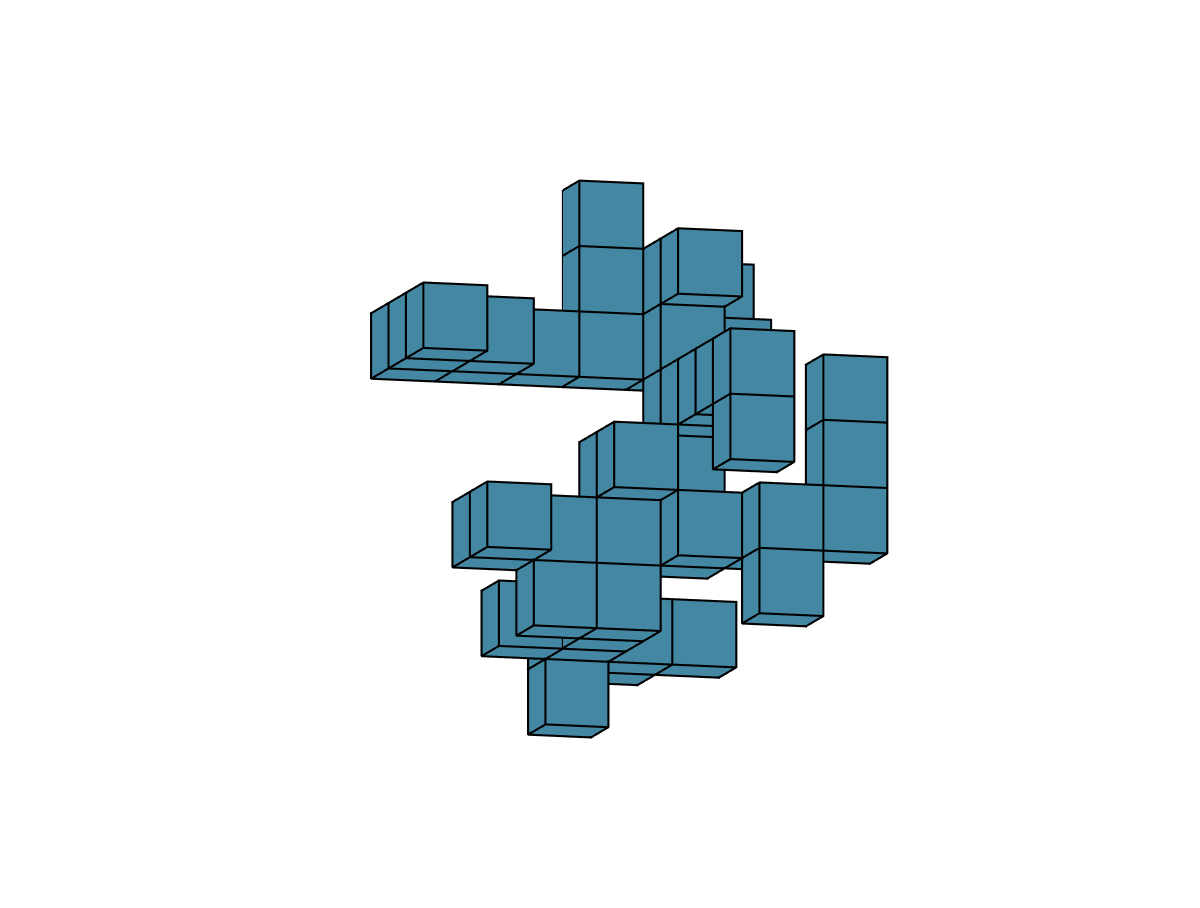
\includegraphics[scale=0.4]{./figures/fig_NC50_sample_compare}
	\caption{Sample aggregate model with 50 cubes for domain size comparison.}
	\label{fig_NC50_sample_compare}
\end{center}
\end{figure}


Domain size variation with fifty cubes.
\begin{figure}[ht]
	\begin{center}
		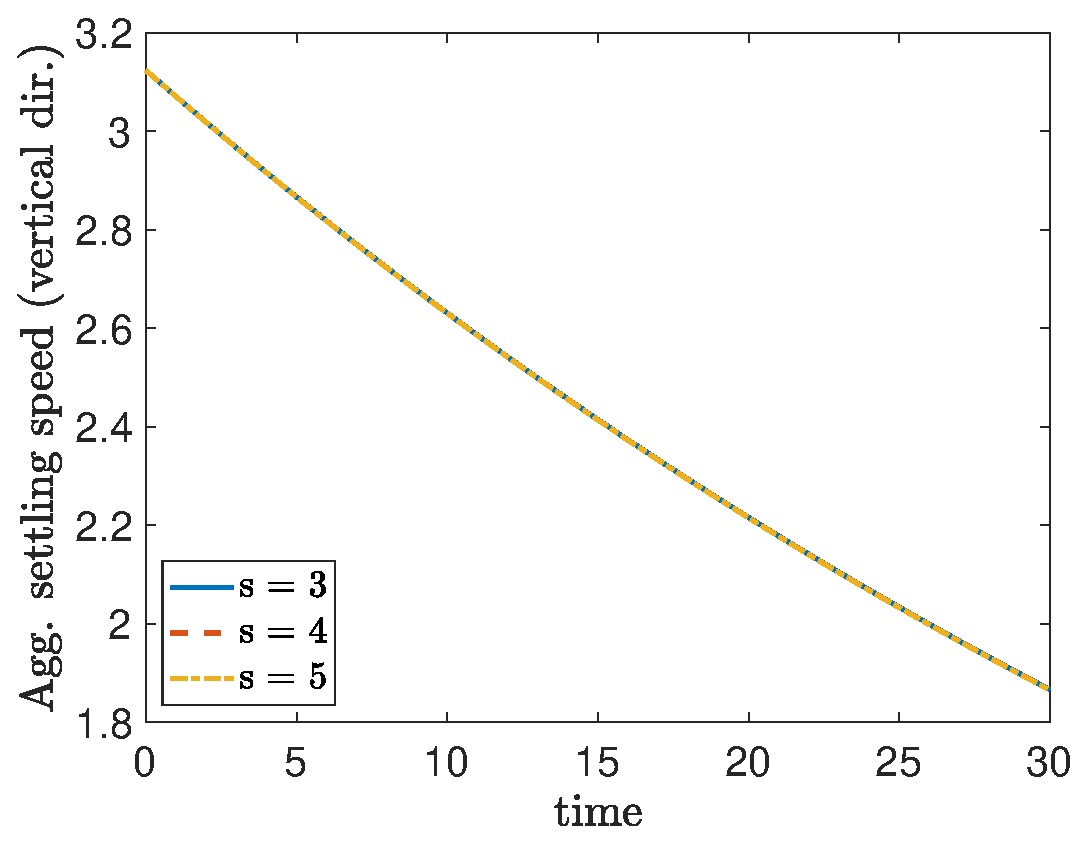
\includegraphics[scale=0.25]{./figures/fig_NC50_s_Ua3_all}
		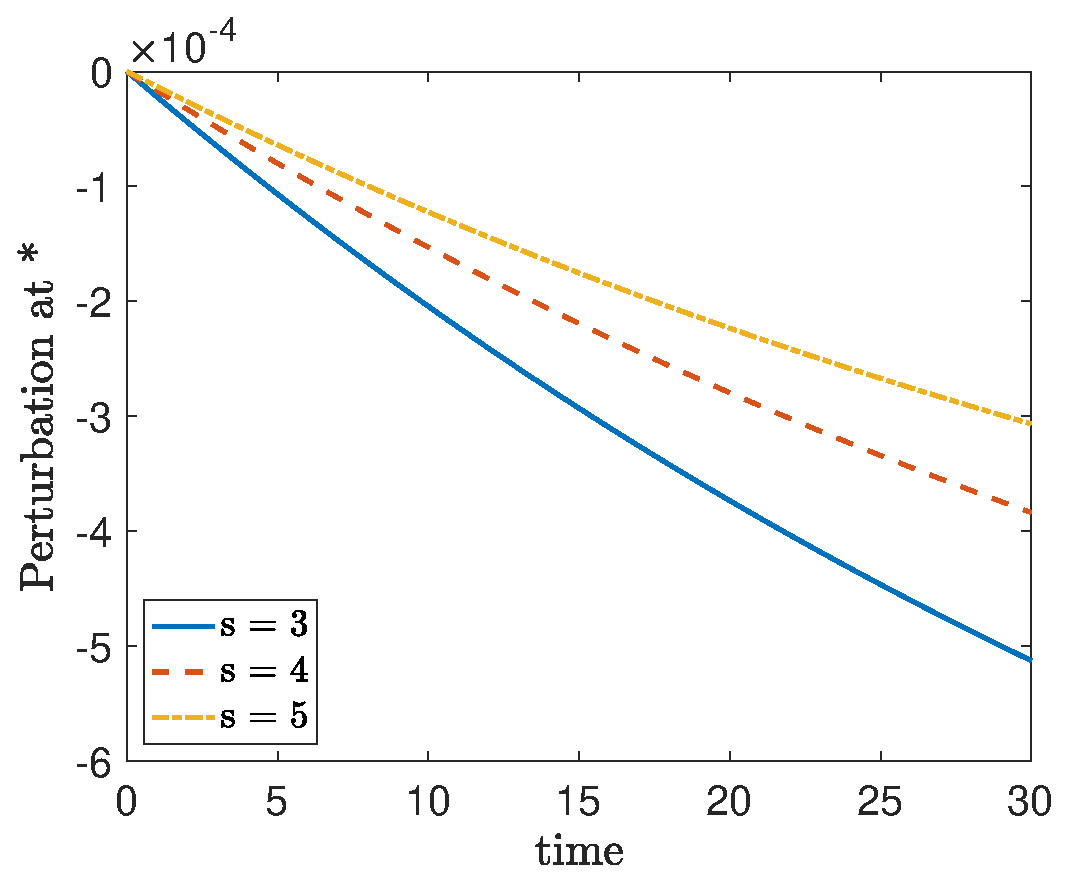
\includegraphics[scale=0.25]{./figures/fig_NC50_s_C_all}
		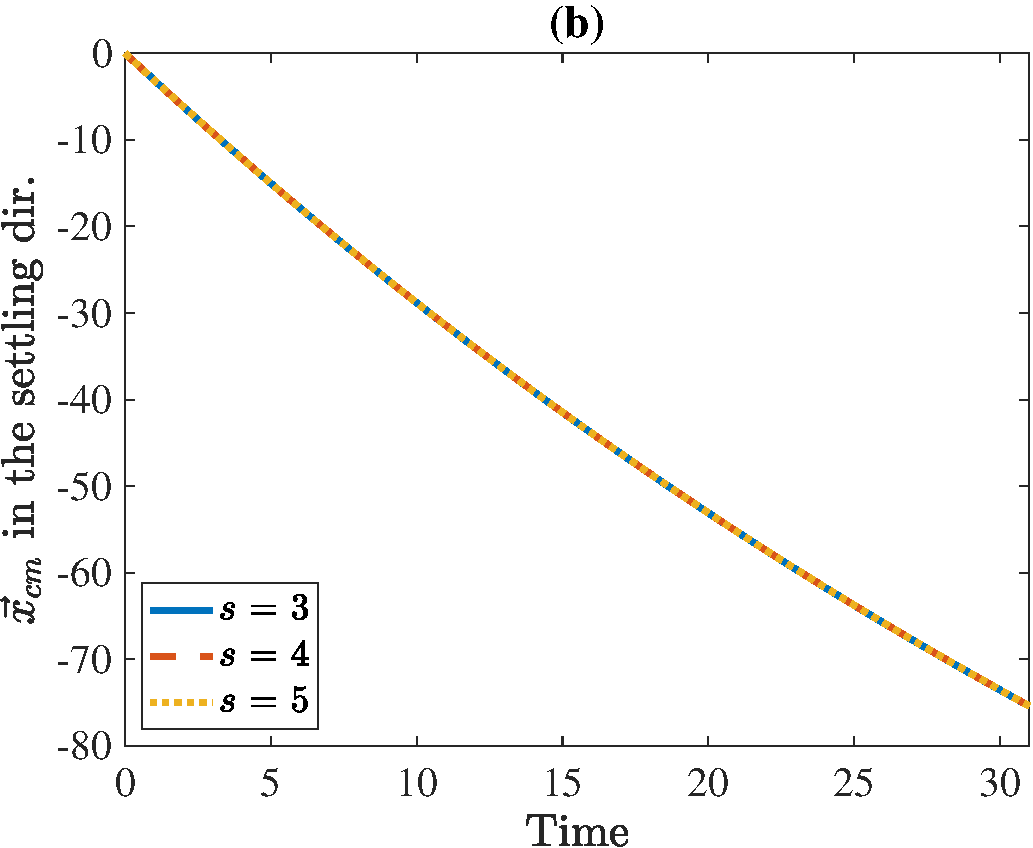
\includegraphics[scale=0.25]{./figures/fig_NC50_s_cm3_all}
		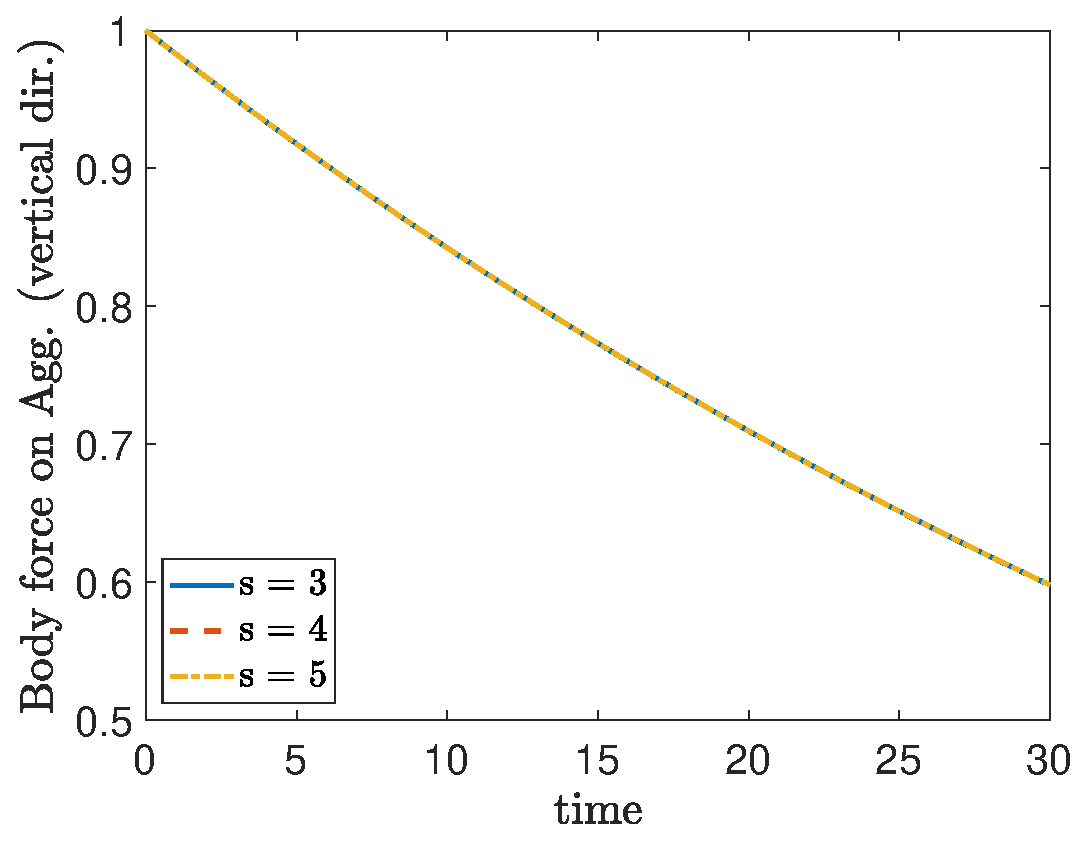
\includegraphics[scale=0.25]{./figures/fig_NC50_s_Fo3_all}
	\caption{Considering an aggregate with fifty cubes, compare various domain sizes $\Delta s = 3, \ 4, \ 5$ in the step sizes $\Delta t = 0.5$ with $\Delta x = 1$.}
	\label{fig_NC50_compare_s}
\end{center}
\end{figure}


\clearpage
\section{Simultation results}
Concerning the potential stability issue, we keep the $\Delta t = 0.5$ and $\Delta x =1$ for further simulations. We also choose to use the domain scaling factor as $s = 5$ to mimic an infinite fluid setting. For the background fluid stratification strength, $\gamma$, which was introduced in equation (\ref{eq_rho_bg}), we suppose the largest aggregate, which is made with a hundred cubes, travels about ten times longer than its radius. As we find the maximum radius of an aggregate composed of $100$ cubes is approximately $16$, we expect this aggregate to settle until the vertical level $z_B = -160$, assuming the initial vertical level of the aggregate is zero. At the location, equation (\ref{eq_rho_bg}) tells us to have background fluid density 
\[
\rho_{bg} = \rho_0 (1-\gamma z_B) =	\rho_0 (1+160\gamma).
\]
Meanwhile, we want the aggregate reaches a neutral buoyancy. To see this, we assume the initial aggregate density, when its fluid portion is $\rho_0$, is equal to the background fluid density after stop settling, i.e., $\rho_a = \rho_{bg}$. After calculation, we find the $\gamma \approx 10^{-4}$. We thus use this value for our simulations by default. We will observe different $\gamma$ values if our time allows. 


\begin{itemize}

	\item We have two different aggregate simulations for $NC = 100$.
	\item Last week, I submitted $NC = 50$ four more cases --> got kicked out because of memory issue. 
	\item Timing results -> how long it takes? Get the Pinnacles information.
	\item NC = 30 is running 
	\item What kind of graph do we want to get? 
	\item NC = 1, 10, 30, 50, 100? See the differences? 
	\item Some snapshots? 
	\item Aggregate models that are used to get the data? (different shapes)
\end{itemize}
\section{Discussions (Conclusion)}
What did you do? 
\\
What did we learn?
\\
How can we contribute to aid research in the carbon cycle/marine aggregate? 
\\
What information we can give them?
\\
Any limitation?
\\
Future potential direction?
\\
Are you going to publish this? 